\documentclass[10pt,colorlinks]{beamer}
  % compress
  %\documentclass[handout,xcolot=pdftex,dvipsnames,table]{beamer}
\definecolor{mybg}{RGB}{255,255,204}
\usepackage{minted}
\usepackage{graphicx}
\usepackage[english]{babel}
\usepackage[utf8x]{inputenc}
\usepackage{amsmath}


 \usepackage{beamerthemesplit}

%\usemintedstyle{trac}

\mode<presentation>
\setbeamercovered{invisible}
\usetheme{Warsaw}
\usecolortheme{dolphin}

\usefonttheme{serif}







% Delete this, if you do not want the table of contents to pop up at
% the beginning of each subsection:
\AtBeginSection[]
{
  \begin{frame}<beamer,allowframebreaks>{Outline}
    \tableofcontents[currentsection]
  \end{frame}
}



\title{ Python in a Nutshell}
\subtitle
{Part III: Introduction to SciPy and SimPy} % (optional)


\author[Velasco and Perera]{Manel Velasco,\inst{1} PhD and Alexandre Perera,\inst{1}$^{,}$\inst{2} PhD}

\institute[UPC] % (optional, but mostly needed)
{
  \inst{1}%
  Departament d'Enginyeria de Sistemes, Automatica i Informatica Industrial (ESAII)  \\
  Universitat Politecnica de Catalunya 
  \and 
  \inst{2}%
   Centro de Investigacion Biomedica en Red en Bioingenieria, Biomateriales y Nanomedicina (CIBER-BBN)  \\
    \href{mailto:Alexandre.Perera@upc.edu}{Alexandre.Perera@upc.edu}~\href{mailto:manel.velasco@upc.edu}{Manel.Velasco@upc.edu}
}
 

\date[Feb, 2013, Learning Python]{Introduction to Python for Engineering and Statistics\\
Febraury, 2013}

 %

\begin{document}


\begin{frame}[plain]
   %  \titlepage
   \maketitle
\end{frame}


\begin{frame}[allowframebreaks]{Contents}
  \tableofcontents
  % You might wish to add the option [pausesections]
 \note[options]{aixo son notes}
\end{frame}

\section{Introduction}

%----------------------------FRAME------------------------------------
\begin{frame}[fragile]\frametitle{SciPy}
\begin{figure}[!htb]
    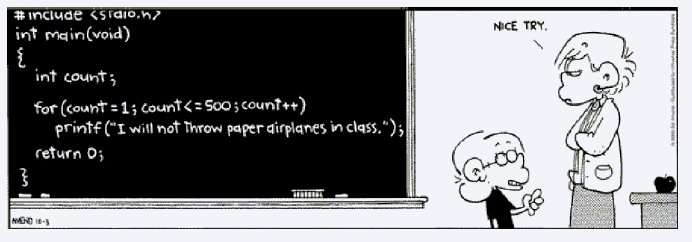
\includegraphics[width=\textwidth]{figs/nicetry}
\end{figure}
\end{frame}
%----------------------------FRAME------------------------------------
\begin{frame}[fragile]\frametitle{Scipy}
Up to now:
\begin{description}
    \item<1->[python]  A general purpose programming language. It is interpreted and dynamically typed and is very suited for interactive work and quick prototyping, while being powerful enough to write large applications in.
    \item<2->[Numpy] A language extension that defines the numerical array and matrix type and basic operations on them.
    \item<3->[matplotlib] A language extension to facilitate plotting. 
    \item<4->[Scipy] Scipy is another language extension that uses numpy to do advanced math, signal processing, optimization, statistics and much more.

\end{description}
\end{frame}

%----------------------------FRAME------------------------------------
\begin{frame}[fragile]\frametitle{History of SciPy}
  \begin{description}
    \item[1995] first, there was \emph{Numeric}, developed by Jim Hugunin
    \item[2001] Several people used Numeric for writing sientific code.  Travis Oliphant, Eric Jones and Pearu Peterson merged their modules in one scientific super package: \emph{SciPy} was born.
    \item[2001-2004] \emph{numarray} was created by Perry Greenfield, Todd Miller and Rick White at the Space Science Telescope Institute as a replacement for Numeric.
    \item[2005] Travis Oliphant took \emph{Numeric} and assambled a multi dimensional array project \emph{SciPy core}. \emph{Numerix} was born but as there was a DSPs company with the same name, \emph{NumPy} was reborn. 
    \item[2006] Guido and Travis discussed which parts of \emph{NumPy} should go into Python standard libraries.  
  \end{description}
\end{frame}
%\section{Importing Data} % (fold)
%\label{sec:Importing Data}

% section Importing Data (end)
\subsection{Input/Output}

%----------------------------FRAME------------------------------------
\begin{frame}[fragile]\frametitle{http://scipy.org}
\begin{figure}[!htb]
    \centering
    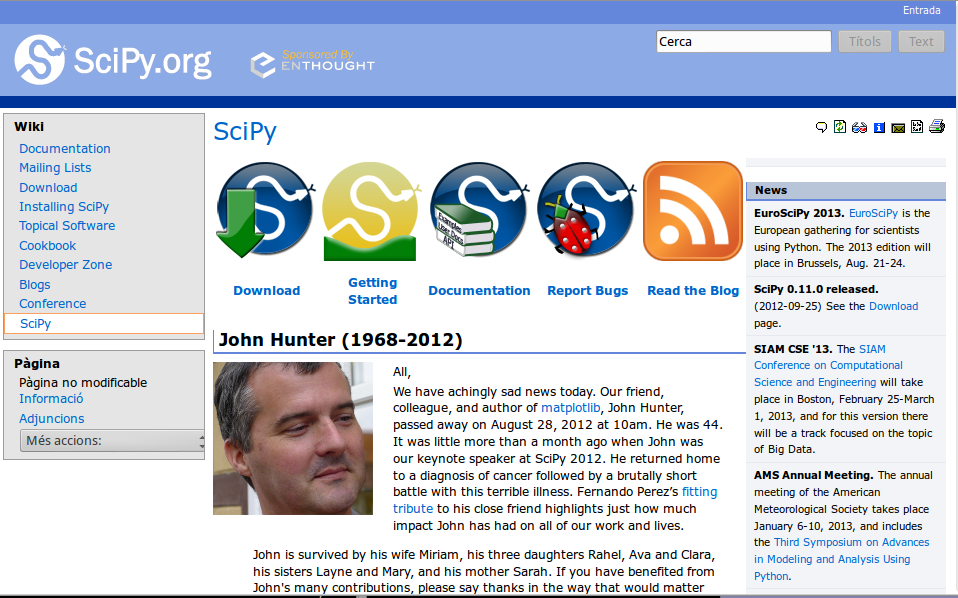
\includegraphics[width=0.9\textwidth]{figs/scipy}
\end{figure}
\end{frame}


%----------------------------FRAME------------------------------------
\begin{frame}[fragile]\frametitle{scipi.io}
Maybe the most common IO in SciPy is to import and export Matlab files using \emph{loadmat/savemat}. In SciPy is easy to write/read them. 
%-------------------------------CODE
{\small
\begin{minted}[bgcolor=mybg,frame=lines,mathescape]{python}
>>> import numpy as np
>>> from scipy import io as spio
>>> py_a = np.ones((2,2))
>>> spio.savemat('ex.mat',{'mat_a': py_a})
>>> py_mat = spio.loadmat('ex.mat')
>>> py_mat['mat_a']
array([[ 1.,  1.],
       [ 1.,  1.]])
\end{minted}

%-------------------------------END CODE
}
%where \verb|struct_as_record| loads the MATLAB structs as python objects rather than numpy structured arrays 
\end{frame}

%----------------------------FRAME------------------------------------
\begin{frame}[fragile]\frametitle{scipy.io}
  \emph{scipy.io} contains modules, classes and functions to read and write data to a variety of formats: 
\begin{description}
    \item[Matlab] \verb|loadmat(file_name[, mdict, appendmat])|
    \item[] \verb|savemat(file_name[, mdict, appendmat])|
    \item[Matrix Market] \href{http://math.nist.gov/MatrixMarket/}{http://math.nist.gov/MatrixMarket/}
    \item[] \verb|mminfo()|, \verb|mmread()| and \verb|mmwrite()|
    \item[Wav] Through \verb|scipy.io.wavfile|.
    \item[] \verb|read()|, \verb|write(file, rate, data)|
    \item[WEKA] ARFF is a text file format which support numerical, string and data values, with support of missing and sparse data.
    \item[] \verb|loadarff()| from \verb|arff| module
    \item[Netcdf] Through \verb|scipy.io.netcdf|
    \item[]  \verb|netcdf_file(filename[, mode, mmap, version])|

\end{description}

\end{frame}

\section{Statistics}
\subsection{First statistics} % (fold)
\label{ssub:First statistics}

%----------------------------FRAME------------------------------------
\begin{frame}[fragile]\frametitle{Statistics}
\begin{figure}[!htb]
    
\includegraphics[width=\textwidth]{figs/nine}
\end{figure}
\end{frame}



% subsubsection First statistics (end)%----------------------------FRAME------------------------------------
\begin{frame}[fragile]\frametitle{Statistics}
    \begin{block}{scipy.stats}
    Contains statistical tools and probabilistic description of random processes.
    \end{block}  
   \pause \begin{block}{numpy.random}
    Contains random number generators for various random process. 
    \end{block}
\end{frame}
%----------------------------FRAME------------------------------------
\begin{frame}[fragile]\frametitle{Main Stats functions}
    \begin{itemize}
        \item scipy.mean()
        \item scipy.var()
        \item scipy.std()
        \item scipy.median()
        \item scipy.scoreatpercentile()
        \item stats.describe() 
        \item stats.mode()
        \item stats.moment()
   \end{itemize}
\end{frame}
\subsection{Probability Distributions} % (fold)
\label{ssub:Probability Distributions}

%----------------------------FRAME------------------------------------
\begin{frame}[fragile]\frametitle{Probability Distributions}
  \begin{block}{}
  \begin{itemize}
      \item  Scipy has functions that deal with several common probability distributions. 
        \item Currently there are 81 continuous probability distributions and 10 discrete distributions. 
        \item These are defined in the scipy.stats sub-package. 
        \item This package also defines several statistical functions.
    \end{itemize} 
  \end{block}
\end{frame}

%----------------------------FRAME------------------------------------
\begin{frame}[fragile]\frametitle{ Prob Distributions}
\begin{block}{Continuous PDFs}
 \begin{description}
      \item[norm] Normal or Gaussian
    \item[chi2] Chi-squared
    \item[t] Student's T
    \item[uniform] Uniform
  \end{description}
\end{block} 

\begin{block}{Discrete PDFs}
\begin{description}
    \item[binom] Binomial
    \item[poisson] Poisson 
\end{description}
\end{block}
\end{frame}


%----------------------------FRAME------------------------------------
\begin{frame}[fragile]\frametitle{Working with PDFs I }
  There are two ways of using probability distribution functions:
\begin{itemize}
    \item Generate a frozen distribution object and then work with the methods of this object.
%-------------------------------CODE
\begin{minted}[bgcolor=mybg,frame=lines,mathescape]{python}
>>> from scipy import stats
>>> N = stats.norm(loc=1, scale=0.5)
\end{minted}

%-------------------------------END CODE
    We can then draw random numbers that follow the distribution we just defined:
%-------------------------------CODE
\begin{minted}[bgcolor=mybg,frame=lines,mathescape]{python}
>>> N.rvs(10)
array([ 1.26041313,  2.05286423,  0.50953812,  0.83991445,  0.69666132,
        0.59828645,  0.90758433,  0.94395294,  1.13686641,  1.04722609])
\end{minted}

%-------------------------------END CODE

\end{itemize}

\end{frame}

%----------------------------FRAME------------------------------------
\begin{frame}[fragile]\frametitle{Working with PDFs II}
Alternatively: 
\begin{itemize}
    \item Use functions in the appropriate class by always passing the parameters that define the distribution, when calling functions associated with the distribution.


    \item For example, to draw a random number from a Gaussian or Normal distribution with mean = 2 and standard deviation = 0.2 we can write:
%-------------------------------CODE
\begin{minted}[bgcolor=mybg,frame=lines,mathescape]{python}
>>> from scipy import stats
>>> stats.norm.rvs(loc=2, scale=0.2, size=3)
array([ 1.7615373 ,  1.91174333,  2.18555173])
\end{minted}

%-------------------------------END CODE
\end{itemize}


\end{frame}


%----------------------------FRAME------------------------------------
\begin{frame}[fragile]\frametitle{stats.describe()}
  %-------------------------------CODE
{ \small
\begin{minted}[bgcolor=mybg,frame=lines,mathescape]{python}
>>> from scipy import stats
>>> R = stats.norm.rvs(loc = 1, scale=0.5, size=1000)
>>> n, min_max, mean, var, skew, kurt = stats.describe(R)
>>> print("Number of elements: {0:d}".format(n))
Number of elements: 1000
>>> print("Minimum: {0:8.6f} Maximum: {1:8.6f}".format(min_max[0], min_max[1]))
Minimum: -0.302407 Maximum: 2.508948
>>> print("Mean: {0:8.6f}".format(mean))
Mean: 0.985060
>>> print("Variance: {0:8.6f}".format(var))
Variance: 0.247292
>>> print("Skew : {0:8.6f}".format(skew))
Skew : 0.058949
>>> print("Kurtosis: {0:8.6f}".format(kurt))
Kurtosis: -0.237082
\end{minted}

}
  %-------------------------------END CODE
\end{frame}


%----------------------------FRAME------------------------------------
\begin{frame}[fragile]\frametitle{Working with PDFs III}
Similarly, the value of the PDF at any value of the variate can be obtained using the function \verb|pdf| of the concerned distribution,
%-------------------------------CODE
\begin{minted}[bgcolor=mybg,frame=lines,mathescape]{python}
>>> stats.norm(1,loc=2,scale=0.2)
<scipy.stats.distributions.rv_frozen object at 0x30f2ad0>
\end{minted}

%-------------------------------END CODE
We can also pass an array of values to this function, to get the PDF at the specified values of the variate:
%-------------------------------CODE
\begin{minted}[bgcolor=mybg,frame=lines,mathescape]{python}
>>> N = stats.norm(loc=2, scale=0.2)
>>> N.pdf([-1,2])
array([  2.76535477e-49,   1.99471140e+00])
\end{minted}

%-------------------------------END CODE   
\end{frame}


%----------------------------FRAME------------------------------------
\begin{frame}[fragile]\frametitle{Multivariate random processes}
\begin{block}{Multivariate Random Processes}
Are provided by the \verb|np.random.multivariate| family.
\end{block}
\begin{block}{}
Could you create and plot a multivariate normal with:
\begin{align}
       \vec \mu & = (0, 0) \\
        \Sigma & = \left( \begin{array}{ccc}
            1 & 0.5 \\
            0.5 & 1
        \end{array} \right)
\end{align}
\end{block}

\end{frame}
%----------------------------FRAME 2 cols------------------------------
\begin{frame}[fragile]\frametitle{Solution}
\begin{columns}[c]
\column{0.5\textwidth}
%-------------------------------CODE
\small 
\begin{minted}[bgcolor=mybg,frame=lines,mathescape]{python}
mean = [0,0]
cov = [[1,0.5],[0.5,1]]
import matplotlib.pyplot as plt
x,y = \
    np.random.multivariate_normal(\
        mean,cov,500).T
plt.plot(x,y,'bo') 
plt.axis('equal')
\end{minted}

%-------------------------------END CODE
\column{0.5\textwidth}
%-------------------------------CODE
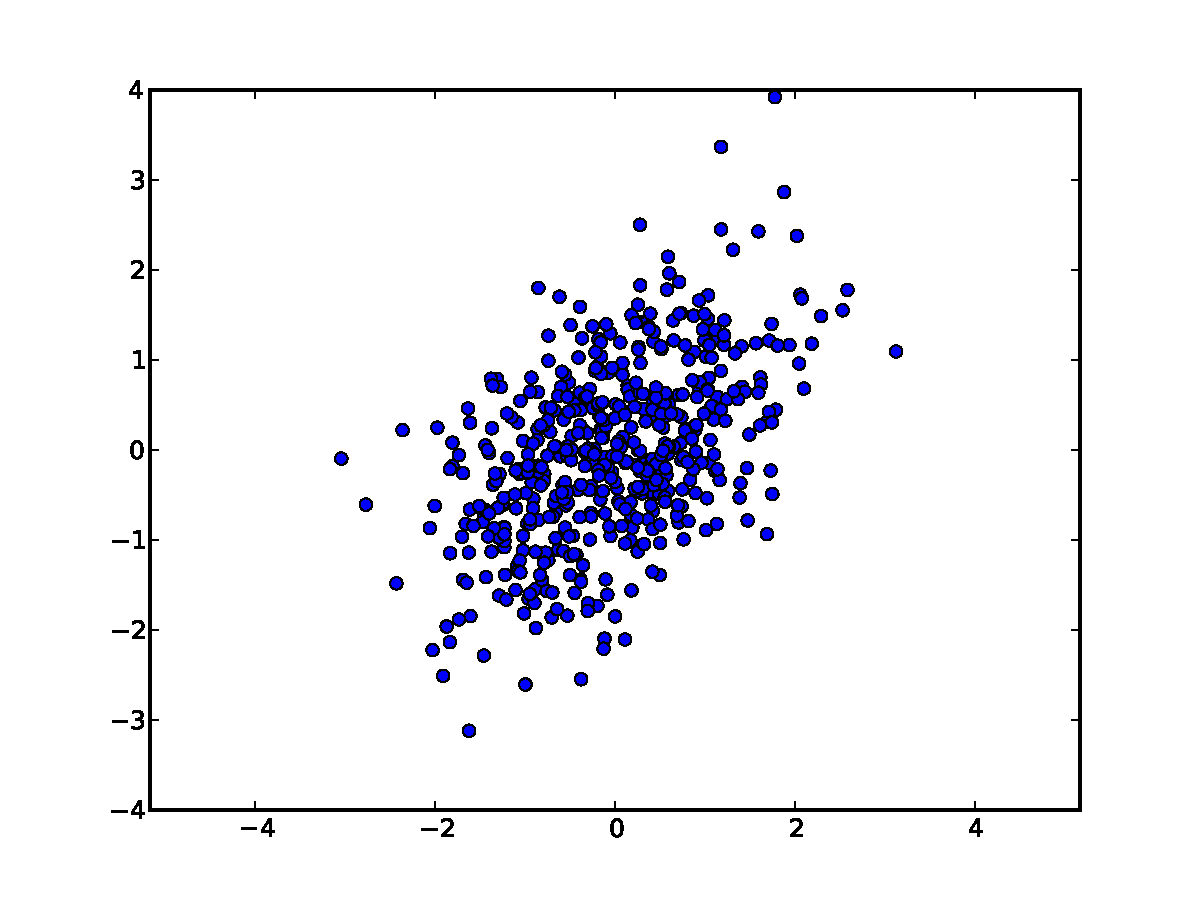
\includegraphics[width=\textwidth]{plwfigis/CursP_3_figure9}

%-------------------------------END CODE
\end{columns}
\end{frame}


%----------------------------FRAME------------------------------------
%\begin{frame}[fragile]\frametitle{Probability Mass Functions}
%For discrete variates the probability mass function (PMF) gives the probability of the variate having a value x.
%For example, for a binomial distribution with $p = 0.7$ and number of trials $n = 5$ we can calculate the PMF using the following:  
%-------------------------------CODE
%<<term=TRUE>>=
%tries = range(10)
%print(stats.binom.pmf(tries,5,0.7))
%
%%-------------------------------END CODE
%\end{frame}
\subsection{Density Estimation} % (fold)
\label{sub:Density Estimation}

% subsection Density Estimation (end)
%----------------------------FRAME------------------------------------
\begin{frame}[fragile]\frametitle{Density Estimation}
  Let's generate a random process and estimate its probability density function (PDF):
%-------------------------------CODE
\begin{minted}[bgcolor=mybg,frame=lines,mathescape]{python}
>>> x = np.random.normal(size=2000)
>>> cuts = np.arange(-6,6)
>>> cuts
array([-6, -5, -4, -3, -2, -1,  0,  1,  2,  3,  4,  5])
>>> hist = np.histogram(x, bins=cuts, normed=True)[0]
>>> bins = (cuts[1:] + cuts[:-1])/2. 
>>> bins 
array([-5.5, -4.5, -3.5, -2.5, -1.5, -0.5,  0.5,  1.5,  2.5,  3.5,  4.5])
\end{minted}

%-------------------------------END CODE
\end{frame}

%%
%import matplotlib
%matplotlib.rcParams.update({'figure.figsize' : (4,2),
%                       'savefig.dpi': 200,
%                        'font.size' : 10 })
%
%----------------------------FRAME------------------------------------
\begin{frame}[fragile]\frametitle{Density Estimation}


\begin{columns}[c]
\column{0.5\textwidth}
%-------------------------------CODE
\begin{minted}[bgcolor=mybg,frame=lines,mathescape]{python}
from scipy import stats
import matplotlib.pyplot as pl
x_pdf = stats.norm.pdf(bins)
pl.plot(bins,hist)
pl.plot(bins,x_pdf)
\end{minted}

%-------------------------------END CODE
\column{0.5\textwidth}
%-------------------------------CODE
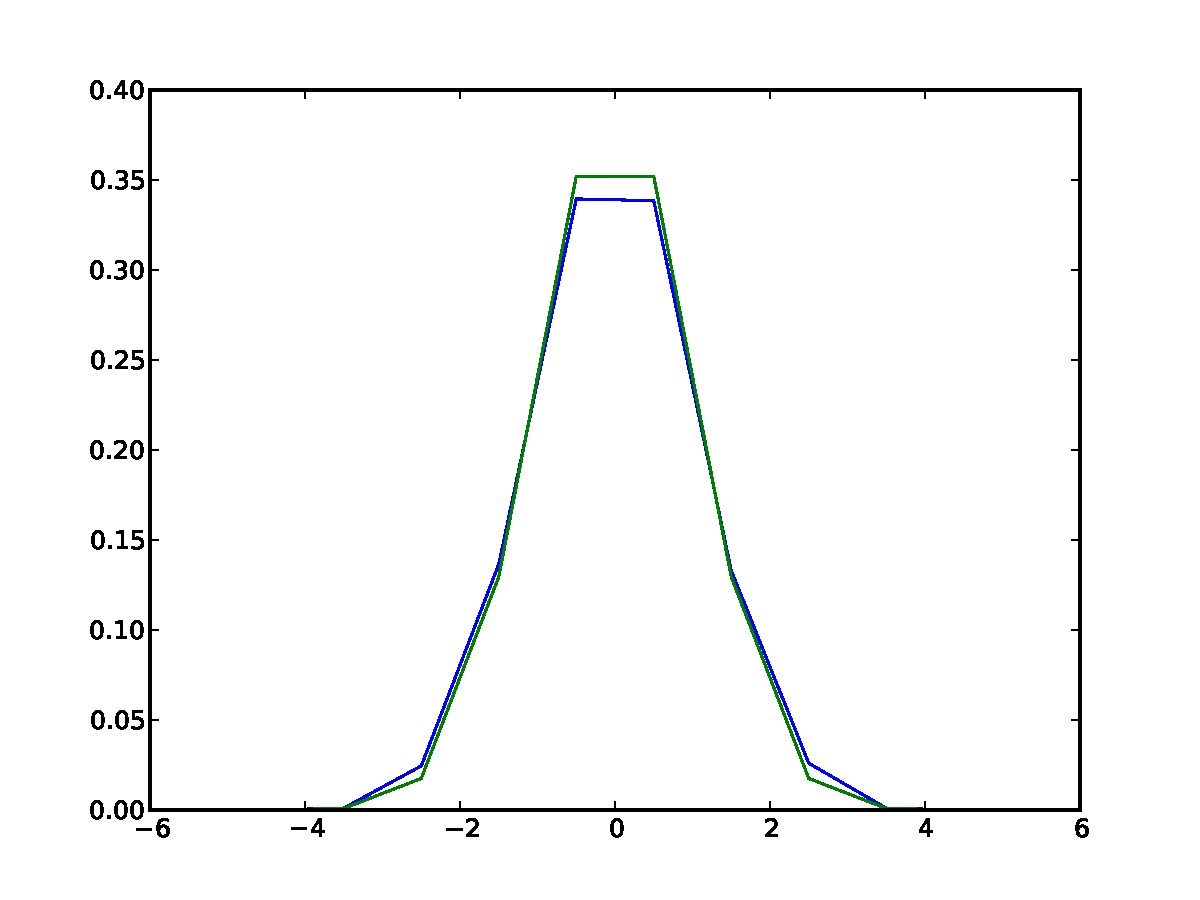
\includegraphics[width=\textwidth]{plwfigis/CursP_3_figure12}

%-------------------------------END CODE
\end{columns}
\end{frame}

%----------------------------FRAME------------------------------------
\begin{frame}\frametitle{Exercise}
  \begin{block}{Exercise}
  Generate a realization of 1000 samples following a Poisson distribution with a parameter of your choice.
 \begin{itemize}
     \item Search for the Poisson methods documentation. Can you estimate the parameter of your own distribution?
 \end{itemize}
  \end{block}
\end{frame}


%----------------------------FRAME------------------------------------
\begin{frame}[fragile]\frametitle{Solution}
\begin{block}{Poisson Probability Mass Distribution}
\begin{align}
    f_{Poiss}( \lambda ) &= \frac{\lambda^k e^{- \lambda}}{k!}\\
\lambda & = E(X)
\end{align}
\end{block}
%-------------------------------CODE
\begin{minted}[bgcolor=mybg,frame=lines,mathescape]{python}
>>> from pylab import plot,show,hist,figure,title
>>> from scipy.stats import poisson
>>> mu = 2.4
>>> R = poisson.rvs(mu, loc=0, size=1000)
>>> print("Mean: {0:1.2f}".format( R.mean() ) ) 
Mean: 2.45
\end{minted}

Note that there also SciPy variants, \verb|scipy.mean()|, \verb|scipy.std()|.
%-------------------------------END CODE
\end{frame}

%----------------------------FRAME------------------------------------
\begin{frame}[fragile]\frametitle{Fitting}
    Distribution fitting is the procedure of selecting a statistical distribution that best fits to a dataset generated by some random process. In this post we will see how to fit a distribution using the techniques implemented in the Scipy library. 

%-------------------------------CODE
\small
\begin{minted}[bgcolor=mybg,frame=lines,mathescape]{python}
>>> from scipy.stats import norm
>>> from numpy import linspace
>>> from pylab import plot,show,hist,figure,title
>>> 
>>> data = norm.rvs(loc=0, scale=1, size=150) 
>>> param = norm.fit(data)
>>> param
(-0.095173366943996918, 1.0003376318003636)
>>> x = linspace(-5,5,100)
>>> pdf_fitted = norm.pdf(x, loc=param[0], scale=param[1])
>>> pdf = norm.pdf(x)
\end{minted}

%-------------------------------END CODE
%----------------------------FRAME------------------------------------
 
\end{frame}
\begin{frame}[fragile]\frametitle{Fitting}

\begin{columns}[c]
 \column{0.5\textwidth}
 % -------------------------------CODE
\begin{minted}[bgcolor=mybg,frame=lines,mathescape]{python}
title('Normal distribution')
plot(x,
    pdf_fitted,'r-',
    x,pdf,'b-')
hist(data,normed=1,alpha=.3)
\end{minted}

%
\column{0.5\textwidth}
%-------------------------------CODE
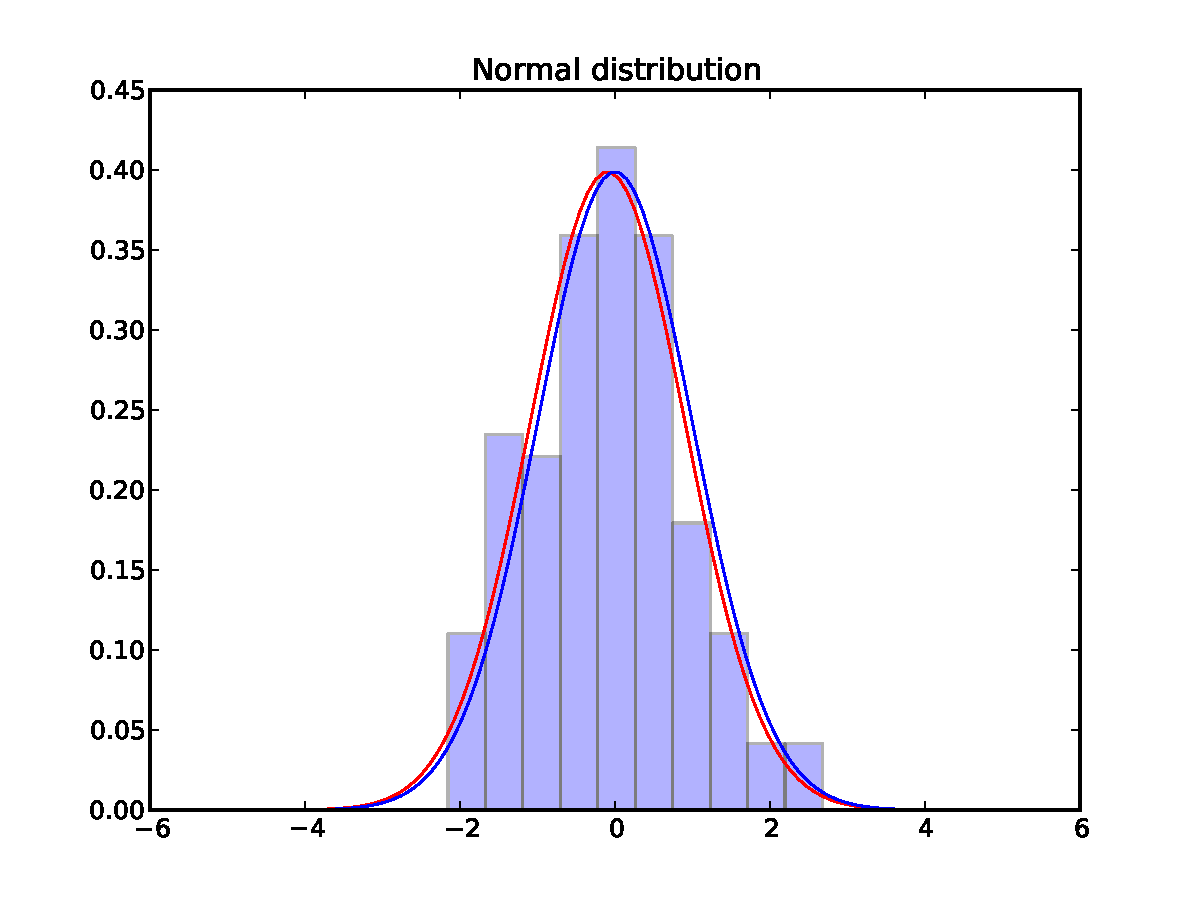
\includegraphics[width=\textwidth]{plwfigis/CursP_3_figure16}

%-------------------------------END CODE   
\end{columns}    
\end{frame}

% subsubsection Probability Distributions (end)

\subsection{Statistical Testing} % (fold)
\label{sub:Statistical Testing}

%----------------------------FRAME------------------------------------
\begin{frame}[fragile]\frametitle{Statistics made easy}
\begin{figure}[!htb]
    \centering
    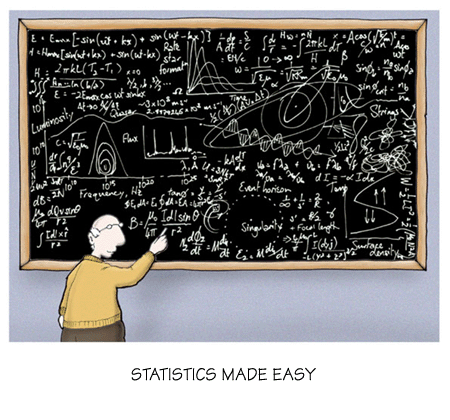
\includegraphics[width=0.7\textwidth]{figs/statisticsmadeeasy}
\end{figure}
\end{frame}


%----------------------------FRAME------------------------------------
\begin{frame}[fragile]\frametitle{Contingency tables}
%-------------------------------CODE
\begin{minted}[bgcolor=mybg,frame=lines,mathescape]{python}
>>> from scipy.stats.contingency import expected_freq 
>>> obs = np.array([[10,20,10],[20,20,10]])
>>> obs
array([[10, 20, 10],
       [20, 20, 10]])
\end{minted}

%-------------------------------END CODE  
\end{frame}

%----------------------------FRAME------------------------------------
\begin{frame}[fragile]\frametitle{$\chi^2$-test}
This function computes the chi-square statistic and p-value for the hypothesis test of independence of the observed frequencies in the contingency table observed. 
%-------------------------------CODE
\begin{minted}[bgcolor=mybg,frame=lines,mathescape]{python}
>>> from scipy import stats
>>> stats.chi2_contingency(obs)
(2.2499999999999991, 0.32465246735834991, 2, array([[ 13.33333333,  17.77777778,   8.88888889],
       [ 16.66666667,  22.22222222,  11.11111111]]))
\end{minted}

%-------------------------------END CODE  

\end{frame}
% subsection Statistical Testing (end)

%----------------------------FRAME------------------------------------
\begin{frame}[fragile]\frametitle{Fisher exact test}
 \begin{block}{Example}
 Say we spend a few days counting whales and sharks in the Atlantic and Indian oceans. In the Atlantic ocean we find 8 whales and 0 shark, in the Indian ocean 2 whales and 5 sharks. Then our contingency table is:
\begin{center}
    
\begin{tabular}{ l c r }
   & Atlantic & Indian \\
  whales & 8 & 2 \\
  sharks & 0 & 5 \\
\end{tabular}
\end{center}
%-------------------------------CODE
 \end{block}
\begin{minted}[bgcolor=mybg,frame=lines,mathescape]{python}
>>> oddsratio, pvalue = stats.fisher_exact([[8, 2], [1, 5]])
>>> pvalue
0.034965034965034919
\end{minted}

%-------------------------------END CODE
\end{frame}

%----------------------------FRAME------------------------------------
\begin{frame}[fragile]\frametitle{t-test}
  \begin{block}{ttest\_ind()}
Calculates the T-test for the means of TWO INDEPENDENT samples of scores. 
  \end{block}
%-------------------------------CODE
\begin{minted}[bgcolor=mybg,frame=lines,mathescape]{python}
>>> rvs1 = stats.norm.rvs(loc=5,scale=10,size=500)
>>> rvs2 = stats.norm.rvs(loc=5,scale=10,size=500)
>>> stats.ttest_ind(rvs1,rvs2)
(-0.24783971064054422, 0.8043094102895727)
>>> rvs3 = stats.norm.rvs(loc=7,scale=10,size=500)
>>> stats.ttest_ind(rvs1,rvs3)
(-2.4139498667262616, 0.015959786513326326)
\end{minted}

%-------------------------------END CODE
\end{frame}



%----------------------------FRAME------------------------------------
\begin{frame}[fragile]\frametitle{t-test (matched)}
  \begin{block}{ttest\_ind()}
Calculates the T-test for the means of TWO MATCHED samples. 
  \end{block}
{ \small
%-------------------------------CODE
\begin{minted}[bgcolor=mybg,frame=lines,mathescape]{python}
>>> rvs1 = stats.norm.rvs(loc=5,scale=10,size=500)
>>> rvs2 = (stats.norm.rvs(loc=5,scale=10,size=500) +
...     stats.norm.rvs(scale=0.2,size=500))
... 
>>> stats.ttest_rel(rvs1,rvs2)
(0.32412677634421311, 0.745977870811666)
>>> rvs3 = (stats.norm.rvs(loc=8,scale=10,size=500) +
...      stats.norm.rvs(scale=0.2,size=500))
... 
>>> stats.ttest_rel(rvs1,rvs3)
(-2.9250238643536557, 0.0036010776543372864)
\end{minted}

}
%-------------------------------END CODE
\end{frame}

%----------------------------FRAME------------------------------------
\begin{frame}[fragile]\frametitle{More tests}
  \begin{description}
      \item[mannwhitneyu()] Computes the Mann-Whitney rank test on samples x and y.
    \item[spearmanr] Calculates a Spearman rank-order correlation coefficient and the p-value.
    \item[pearsonr] Calculates a Pearson correlation coefficient and the p-value for testing.
    \item[f\_oneway] Performs a 1-way ANOVA.
    \item[oneway] Test for equal means in two or more samples from the normal distribution.
    \item[normaltest] Tests whether a sample differs from a normal distribution.
    \item[kruskal] Compute the Kruskal-Wallis H-test for independent samples.
  \end{description}
\end{frame}

%----------------------------FRAME------------------------------------
\begin{frame}[fragile]\frametitle{Plot tests}
  \begin{description}
      \item[probplot] Calculate quantiles for a probability plot against a theoretical distribution. 
  \end{description}
 \begin{columns}[c]
    \column{0.4\textwidth}
\tiny
\begin{minted}[bgcolor=mybg,frame=lines,mathescape]{python}
import scipy.stats as stats
import matplotlib.pyplot as plt 
nsample = 100
np.random.seed(7654321)
ax1 = plt.subplot(221)
x = stats.t.rvs(3, size=nsample)
res = stats.probplot(x, plot=plt)
ax2 = plt.subplot(222)
x = stats.t.rvs(25, size=nsample)
res = stats.probplot(x, plot=plt)
ax3 = plt.subplot(223)
x = stats.norm.rvs(loc=[0,5], scale=[1,1.5],
     size=(nsample/2.,2)).ravel()
res = stats.probplot(x, plot=plt)
ax4 = plt.subplot(224)
x = stats.norm.rvs(loc=0, scale=1, size=nsample)
res = stats.probplot(x, plot=plt)
\end{minted}

\column{0.6\textwidth}
%-------------------------------CODE
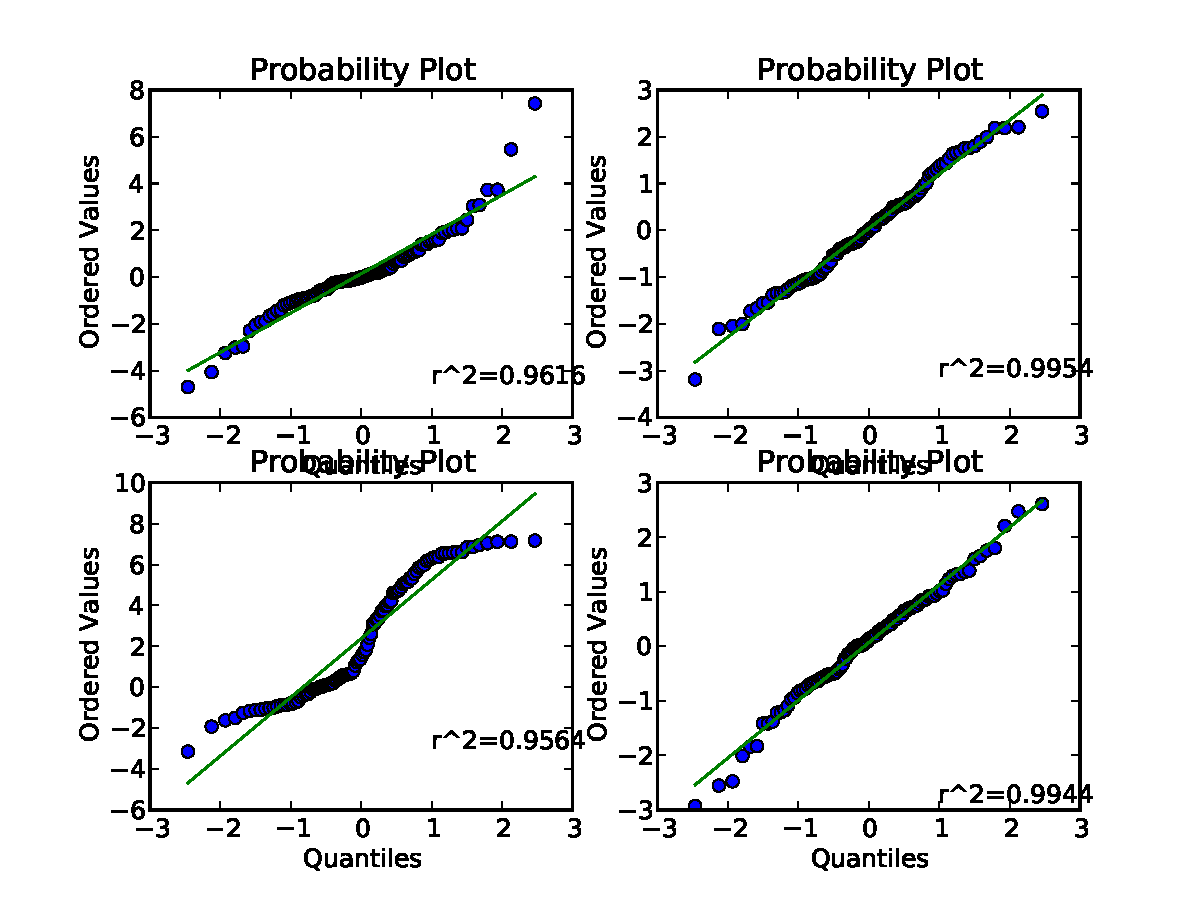
\includegraphics[width=\textwidth]{plwfigis/CursP_3_figure23}

%-------------------------------END CODE
\end{columns}
\end{frame}

\section{Some Calculus} % (fold)
\label{sec:Some Calculus}
\subsection{Linear Algebra}
%----------------------------FRAME------------------------------------
\begin{frame}[fragile]\frametitle{scipy.linalg}
  \begin{block}{}
    The \verb|scipy.linalg| module provides standard linear algebra operations, relying on an underlying efficient implementation (BLAS, LAPACK). Some of the main functions are:
  \end{block}
\begin{description}
    \item[inv] Compute the inverse of a matrix.
    \item[pinv] Compute the (Moore-Penrose) pseudo-inverse of a matrix.
%    \item[lstsq] Least-Squares Solution to $A \cdot x = b$.
    \item[solve] Solve the equation $A\cdot X  = B$  for $X$. 
    \item[det]  Compute the determinant of a matrix.
    \item[norm] Matrix or vector norm.
\end{description}
\end{frame}

%----------------------------FRAME------------------------------------
\begin{frame}[fragile]\frametitle{scipy.linalg}
  \begin{description}
      \item[eig] Solve an ordinary or generalized eigenvalue problem of a square matrix (\verb|eigh()| for complex).
    \item[svd] Singular Value Decomposition.
    \item[orth] Construct an orthonormal basis for the range of A using SVD.
    \item[qr] Compute QR decomposition of a matrix.
    \item[expm] Compute the matrix exponential using Pade approximation. 
    \item[logm] Compute matrix logarithm.
    \item[sinm] Matrix sin/cos/tan. 
    \item[cosm] e.g. $cos(A) = I - \frac{1}{2!}A^2 + \frac{1}{4!}A^4 - \cdots $
    \item[tan]
    \item[funm] Evaluate a matrix function specified by a callable.
  \end{description}
\end{frame}

%----------------------------FRAME------------------------------------
\begin{frame}[fragile]\frametitle{solve()}
  \begin{block}{$A \cdot x = b$}
  Given $a$ and $b$, solve for x.
  \end{block}
%-------------------------------CODE
\begin{minted}[bgcolor=mybg,frame=lines,mathescape]{python}
>>> from scipy import linalg
>>> from numpy import dot
>>> a = np.array([[3,2,0],[1,-1,0],[0,5,1]])
>>> b = np.array([2,4,-1])
>>> x = linalg.solve(a,b)
>>> x
array([ 2., -2.,  9.])
>>> np.dot(a, x) 
array([ 2.,  4., -1.])
\end{minted}

%-------------------------------END CODE
\end{frame}

%----------------------------FRAME------------------------------------
\begin{frame}[fragile]\frametitle{pinv()}
  \begin{block}{pinv()}
  Calculate a generalized inverse of a matrix using a least-squares solver.
  \end{block}
%-------------------------------CODE
\begin{minted}[bgcolor=mybg,frame=lines,mathescape]{python}
>>> a = np.random.randn(5, 3)
>>> B = linalg.pinv(a)
>>> np.allclose(a, dot(a, dot(B, a)))
True
>>> np.allclose(B, dot(B, dot(a, B)))
True
\end{minted}

%-------------------------------END CODE

\end{frame}


%----------------------------FRAME------------------------------------
\begin{frame}[fragile]\frametitle{numpy's allclose() }
  \begin{block}{numpy.allclose()}
  %\pause \begin{block}{np.allclose()}
Returns True if two arrays are element-wise equal within a tolerance.
   \begin{equation}
    abs(a-b) \leq atol + rtol \cdot abs(b)
\end{equation}
\end{block}

\begin{description}
     \item  Relative difference: $rtol \cdot abs(b)$. 
     \item[rtol] Defaults to $1e^{-5}$.
    \item[atol] Defaults to $1e^{-8}$. 
\end{description}
\end{frame}

%----------------------------FRAME------------------------------------
\begin{frame}[fragile]\frametitle{Singular Value Decomposition}
\begin{block}{Matrix Decompositions}
SVD is commonly used in statistics and signal processing. Many other standard decompositions (QR, LU, Cholesky, Schur), as well as solvers for linear systems, are available in scipy.linalg.
\end{block}
%-------------------------------CODE
\begin{minted}[bgcolor=mybg,frame=lines,mathescape]{python}
>>> Mat = np.arange(9).reshape((3, 3)) + np.diag([1, 0, 1])
>>> uMat, S, vMat = linalg.svd(Mat)
>>> S
array([ 14.88982544,   0.45294236,   0.29654967])
\end{minted}

%-------------------------------END CODE
%-------------------------------CODE
\pause 
\begin{minted}[bgcolor=mybg,frame=lines,mathescape]{python}
>>> sMat = np.diag(S)
>>> recMat =  uMat.dot(sMat).dot(vMat)
>>> np.allclose(recMat,Mat)
True
\end{minted}

%-------------------------------END CODE
  
\end{frame}
% section Some Calculus (end)
\subsection{Fast Fourier Transforms}
%----------------------------FRAME------------------------------------
\begin{frame}[fragile]\frametitle{Fast Fourier Transforms}
  \begin{block}{}
  Ok, up to this, boring algebra, I need some action!!
  \end{block}
\pause \begin{block}{FFT through scipy.fftpack}
The scipy.fftpack module allows to compute fast Fourier transforms.
In this example we will:
\begin{itemize}
    \item Generate a noisy signal.
    \item Detect a high frequency component (noise).
    \item Filter this noise in Fourier. 
    \item Plot the filtered signal. 
\end{itemize}
\end{block}
\end{frame}


%----------------------------FRAME------------------------------------
\begin{frame}[fragile]\frametitle{Signal Generation}
  \begin{block}{}
  A typical noisy input may look like the following:
 \end{block}

\begin{minted}[bgcolor=mybg,frame=lines,mathescape]{python}
time_step = 0.02
period = 5.0
time_vector = np.arange(0, 20, time_step)
signal = np.sin(2.0 * np.pi * time_vector / period) + \
 0.4 * np.random.randn(time_vector.size)
\end{minted}

\end{frame}



\begin{frame}[fragile]\frametitle{Signal Generation}

\begin{columns}[c]
  \column{0.5\textwidth}
%-------------------------------CODE
\begin{minted}[bgcolor=mybg,frame=lines,mathescape]{python}
plt.plot(time_vector, signal)
plt.xlabel('Time (s)')
plt.ylabel('Amplitude')
\end{minted}

%-------------------------------END CODE
%-------------------------------END CODE
\column{0.5\textwidth}
%-------------------------------CODE
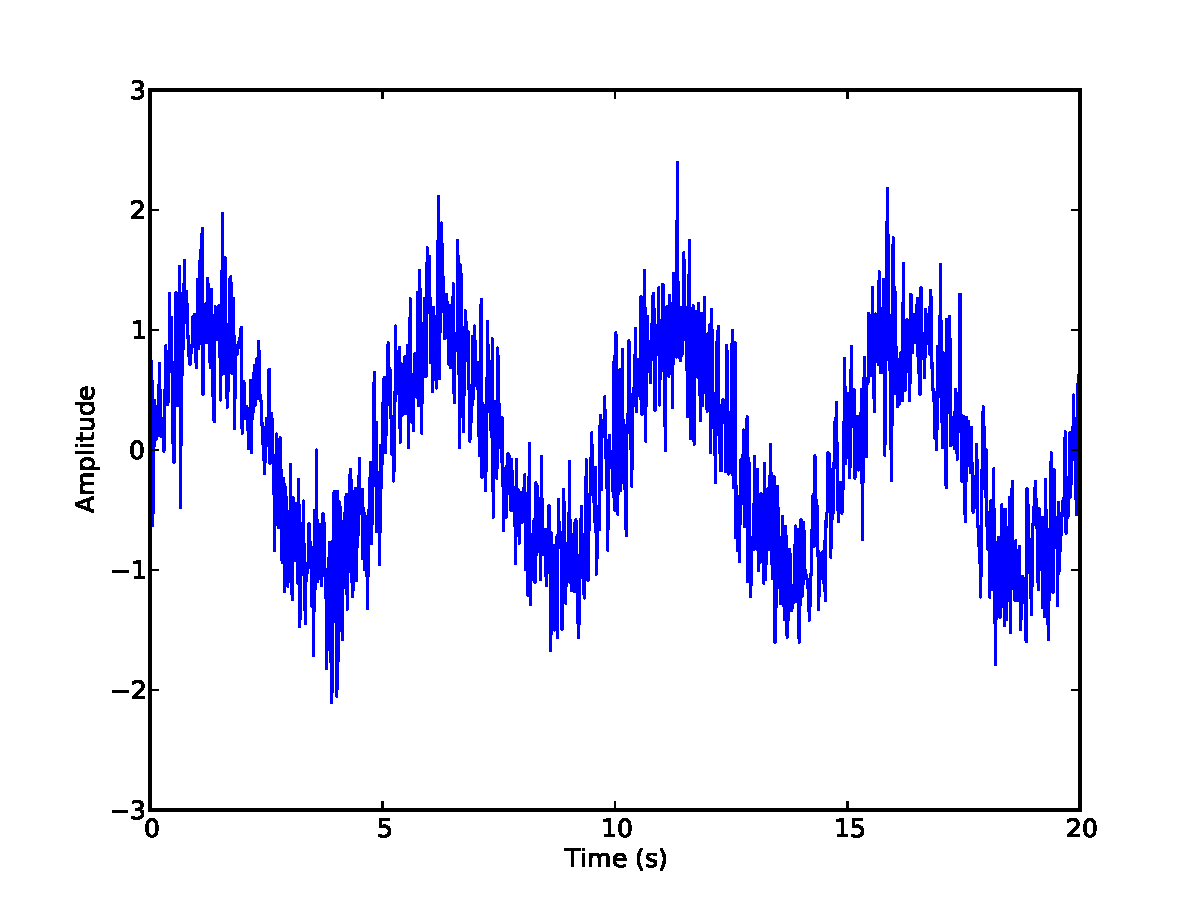
\includegraphics[width=\textwidth]{plwfigis/CursP_3_fft2}

%-------------------------------END CODE
\end{columns}
\end{frame}

%----------------------------FRAME------------------------------------
\begin{frame}[fragile]\frametitle{FFT}
For convenience, we need to first define a vector with the discrete Fourier Transform sample frequencies: 

%-------------------------------CODE
\begin{minted}[bgcolor=mybg,frame=lines,mathescape]{python}
>>> from scipy import fftpack
>>> freqs = fftpack.fftfreq(signal.size, d=time_step)
>>> freqs[0:5]
array([ 0.  ,  0.05,  0.1 ,  0.15,  0.2 ])
>>> freqs[-5:-1] 
array([-0.25, -0.2 , -0.15, -0.1 ])
\end{minted}

%-------------------------------END CODE
And the transformation itself: 
%-------------------------------CODE
\begin{minted}[bgcolor=mybg,frame=lines,mathescape]{python}
>>> sig_fft = fftpack.fft(signal)
\end{minted}

%-------------------------------END CODE
\end{frame}

%----------------------------FRAME------------------------------------
\begin{frame}[fragile]\frametitle{FFT}
We can find the peak on the signal as follows. First select positive frequencies.   

%-------------------------------CODE
\begin{minted}[bgcolor=mybg,frame=lines,mathescape]{python}
>>> ind = np.where(freqs > 0 )
>>> freqs_p = freqs[ind]
>>> signal_abs = np.abs(sig_fft)[ind]
\end{minted}

Then, where do we find the maximum amplitude ?
%-------------------------------CODE
\begin{minted}[bgcolor=mybg,frame=lines,mathescape]{python}
>>> fpeak = freqs_p[signal_abs.argmax()]
>>> print fpeak, 1./period 
0.2 0.2
\end{minted}

%-------------------------------END CODE

\end{frame}

%----------------------------FRAME------------------------------------
\begin{frame}[fragile]\frametitle{FFT}
  
Let's filter the noise above the signal and compute the inverse transform: 

\begin{columns}[c]
    \column{0.5\textwidth}
%-------------------------------CODE
\small 
\begin{minted}[bgcolor=mybg,frame=lines,mathescape]{python}
sig_fft[np.abs(freqs) > fpeak] = 0
main_signal = fftpack.ifft(sig_fft)
plt.figure()
plt.plot(time_vector, signal)
plt.plot(time_vector, 
    main_signal, linewidth=5)
plt.xlabel('Time [s]')
plt.ylabel('Amplitude')
\end{minted}

%-------------------------------END CODE        
    \column{0.5\textwidth}
%-------------------------------CODE
\begin{minted}[bgcolor=mybg,frame=lines,mathescape]{python}
plt.show()
\end{minted}
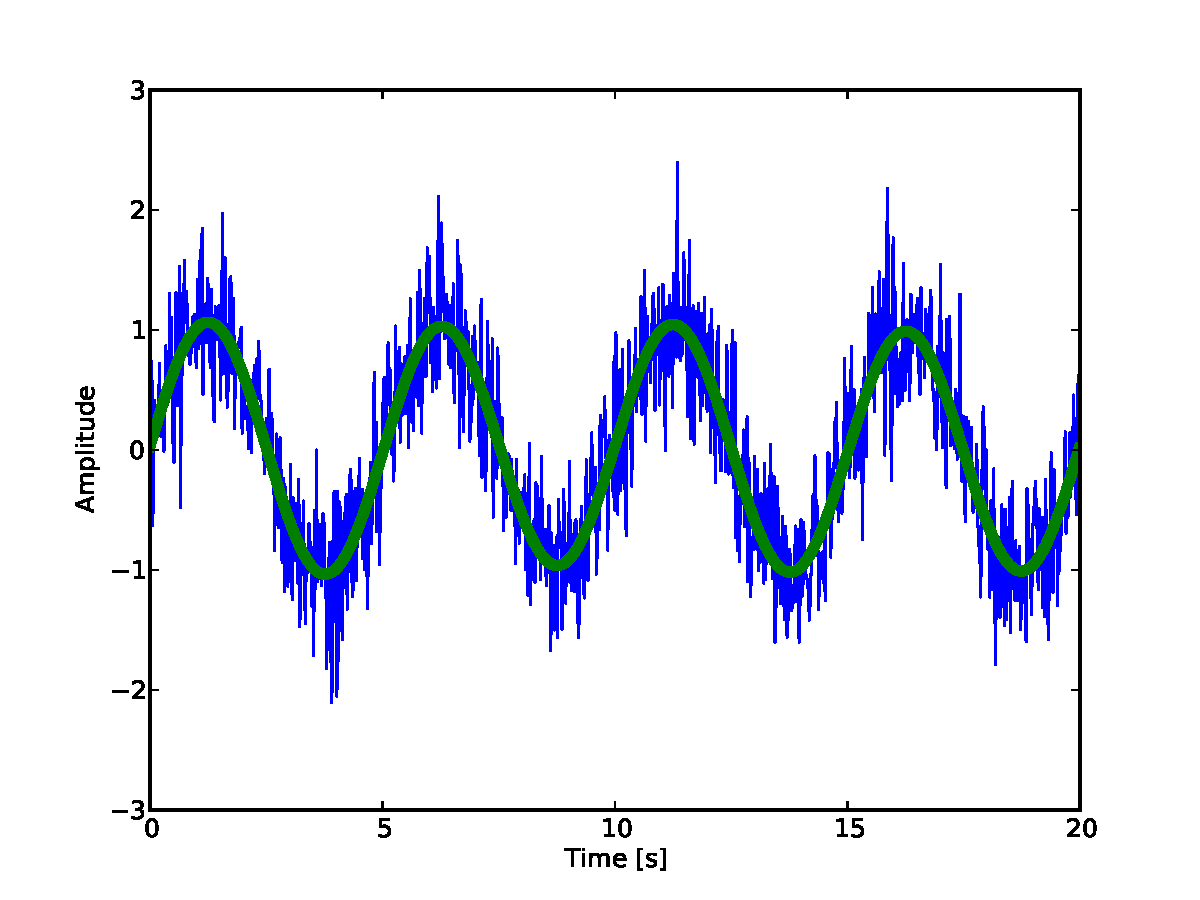
\includegraphics[width=\textwidth]{plwfigis/CursP_3_figure36}

%-------------------------------END CODE
\end{columns}
\end{frame}


%----------------------------FRAME------------------------------------
\begin{frame}[fragile]\frametitle{Challenge!}
Let's consider this noisy image.\tiny{\href{https://www.dropbox.com/s/a73c0lla7qdjqiy/orionnebulaN.jpg}{https://www.dropbox.com/s/a73c0lla7qdjqiy/orionnebulaN.jpg Download link}}

 \begin{columns}[c]

    \column{0.5\textwidth}    
    \begin{figure}[!htb]
      \centering
     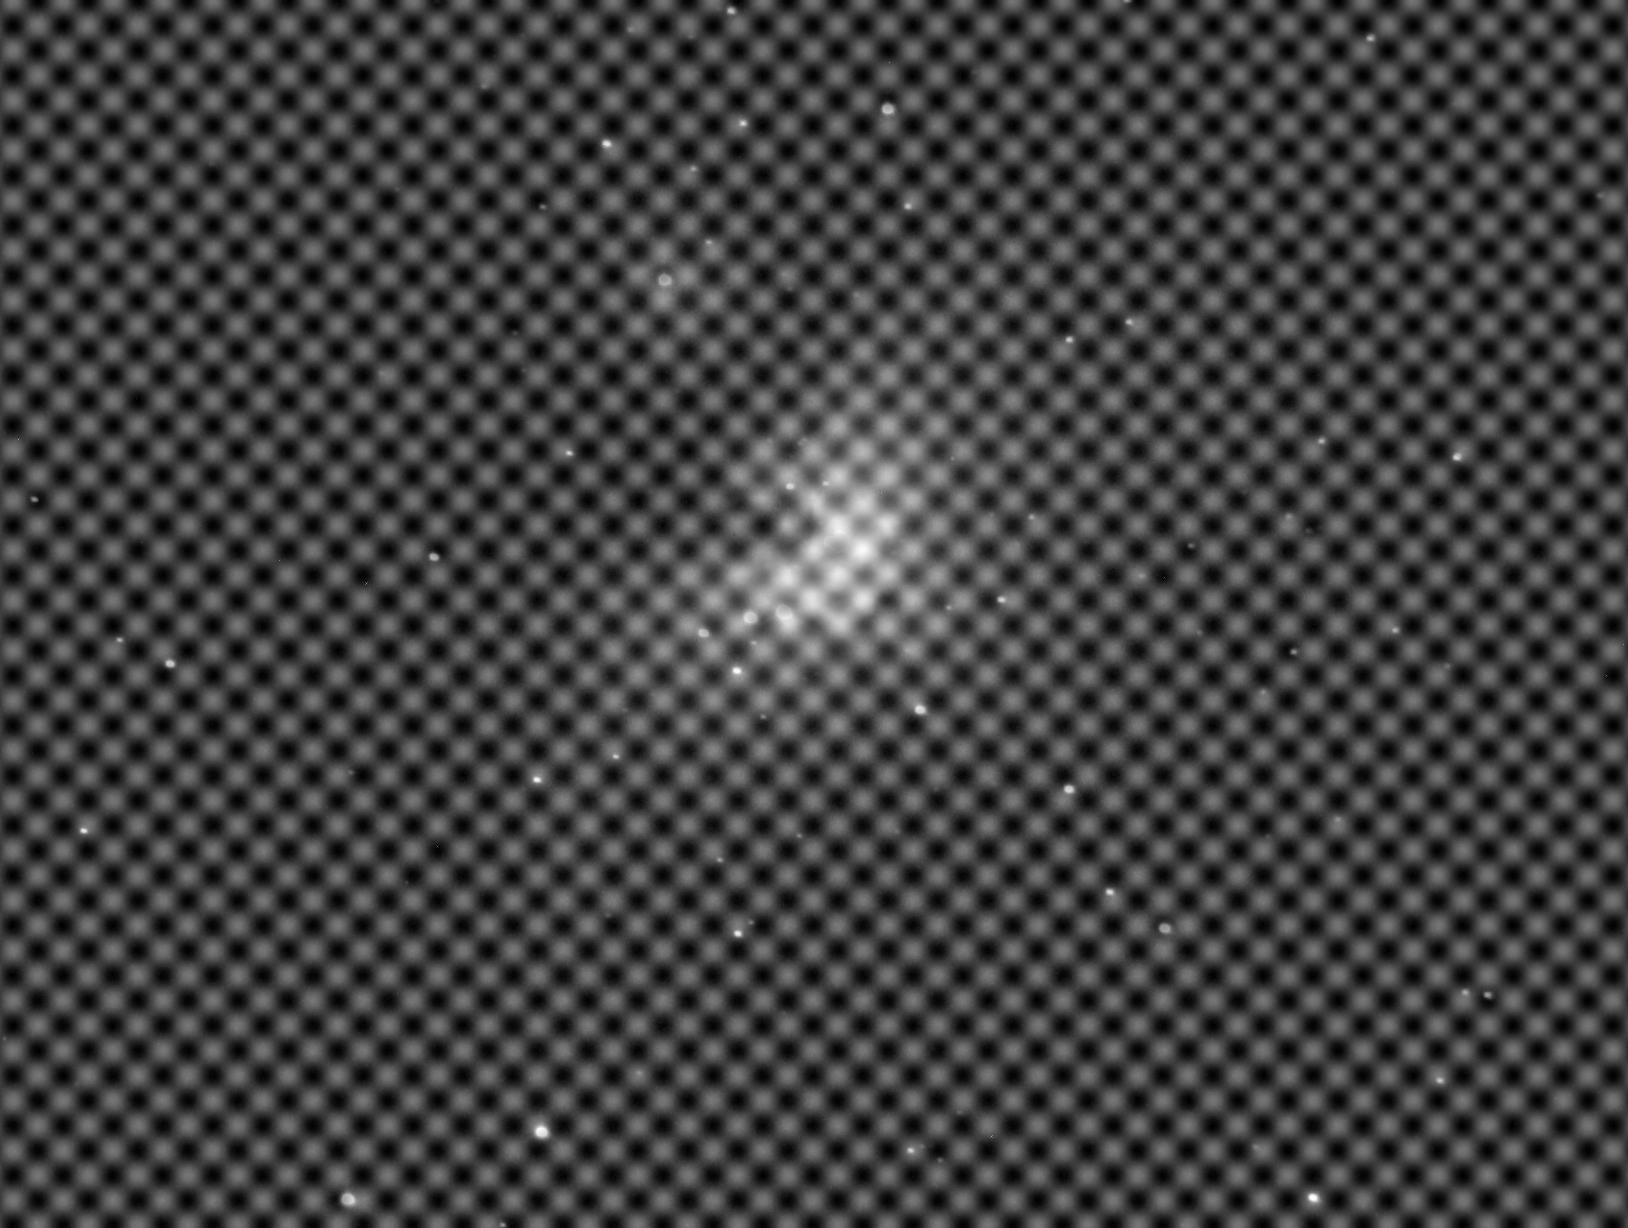
\includegraphics[width=0.6\textwidth]{challenges/orionnebulaN}
     \caption{Picture with periodic noise.}
     \label{fig:}
    \end{figure}
   \column{0.5\textwidth}  
    \begin{block}{}
    Use the 2D FFT implementation in \emph{scipy.fftpack} to remove the noise int the picture:
        \begin{enumerate}
            \item Import the image into ipython through \verb|plt.imread()|
            \item Compute the power spectrum of the Fourier Transform and plot it. 
            \item Cut the high-frequency part zeroing the 2D Fourier Transform matrix. 
             \item Apply the inverse Fourier transform to retrieve the original image.
        \end{enumerate}
    \end{block}
 \end{columns}

\end{frame}




\subsection{Optimization}

%----------------------------FRAME------------------------------------
\begin{frame}[fragile]\frametitle{Optimization}
  \begin{block}{Optimization}
  Optimization is the problem of finding a numerical solution to a minimization or equality.
  \end{block}

\pause \begin{block}{scipy.optimize}
The scipy.optimize module provides useful algorithms for:
\begin{enumerate}
    \item Function minimization (scalar or multi-dimensional)
    \item Curve fitting.
    \item Root finding.
\end{enumerate} 
\end{block}
\end{frame}

%----------------------------FRAME------------------------------------
\begin{frame}[fragile]\frametitle{Finding a Minimum for a Scalar function}
  Let's define the following function:
\begin{equation}
    f(x)=x^2 + 10 sin(x)
\end{equation}
\begin{columns}[c]
    \column{0.5\textwidth}
%-------------------------------CODEA
\small
\begin{minted}[bgcolor=mybg,frame=lines,mathescape]{python}
def f(x):
    return x**2 + 10*np.sin(x)

x = np.arange(-10, 10, 0.1)
plt.plot(x, f(x))  
\end{minted}

%-------------------------------END CODE
\column{0.5\textwidth}
%-------------------------------CODE
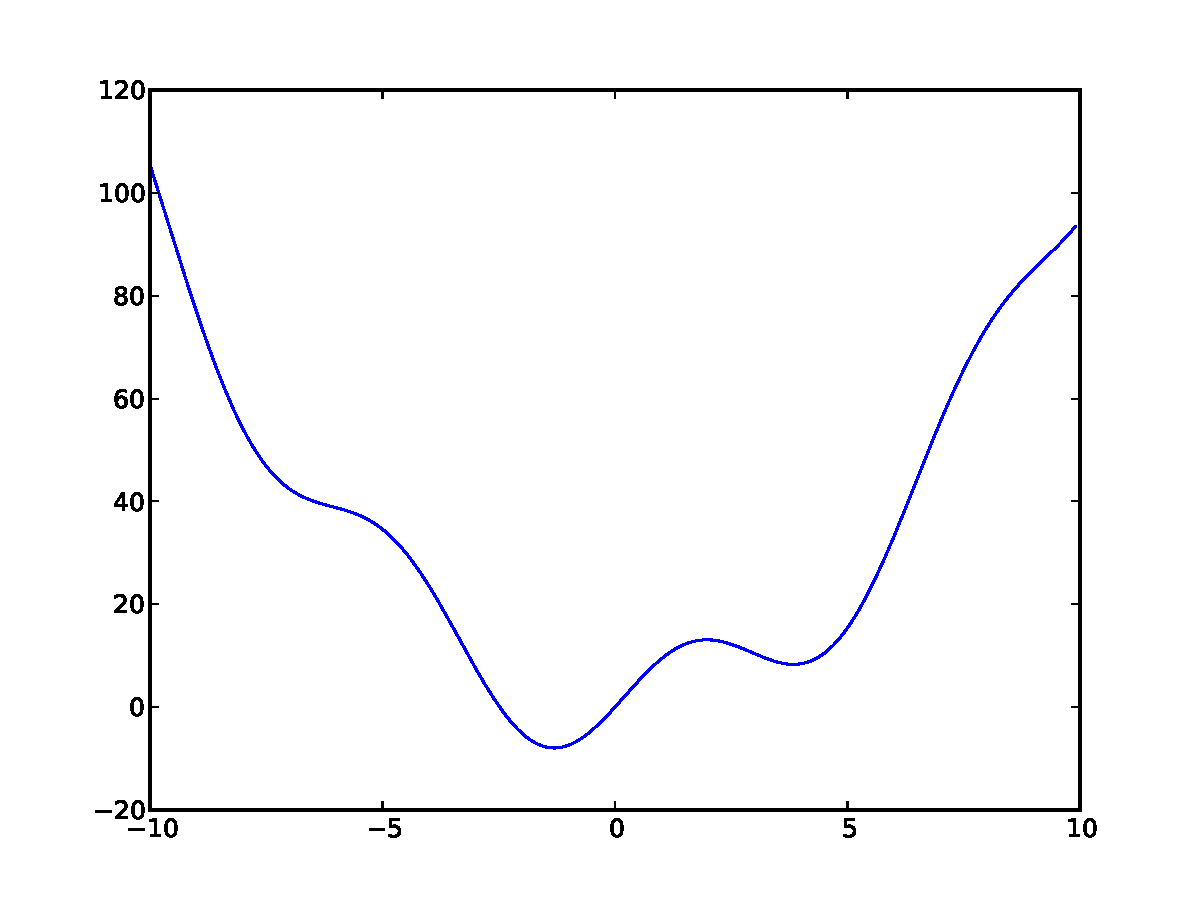
\includegraphics[width=\textwidth]{plwfigis/CursP_3_figure38}

%-------------------------------END CODE
\end{columns}
%-------------------------------END CODE
\end{frame}

%----------------------------FRAME------------------------------------
\begin{frame}[fragile]\frametitle{Finding a Minimum for a Scalar Function}
 The general and efficient way to find a minimum for this function is to conduct a gradient descent starting from a given initial point. The BFGS algorithm is a good way of doing this:
 %-------------------------------CODE
\begin{minted}[bgcolor=mybg,frame=lines,mathescape]{python}
>>> from scipy import optimize 
>>> 
>>> optimize.fmin_bfgs(f, 0)
Optimization terminated successfully.
         Current function value: -7.945823
         Iterations: 5
         Function evaluations: 24
         Gradient evaluations: 8
array([-1.30644003])
\end{minted}

 %-------------------------------END CODE
\end{frame}

%----------------------------FRAME------------------------------------
\begin{frame}[fragile]\frametitle{Brute Force Optimization}

But, watch out! 
%-------------------------------CODE
\begin{minted} [bgcolor=mybg,frame=lines,bgcolor=mybg,frame=lines,bgcolor=mybg,frame=lines,mathescape]{python}
optimize.fmin_tnc(f, 5, disp=0)
array([4.60643939])
\end{minted}

%-------------------------------END CODE
\pause
In case there is no information on the neighborhood - and therefore we have no clues on where to set up the initialization -  we might need to search for a global minimum through brute force.
 %-------------------------------CODE
\begin{minted}[bgcolor=mybg,frame=lines,mathescape]{python}
>>> grid = (-10, 10, 0.1)
>>> xmin_global = optimize.brute(f, (grid,))
>>> xmin_global
array([-1.30641113])
\end{minted}

 %-------------------------------END CODE
\end{frame}

%----------------------------FRAME------------------------------------
\begin{frame}[fragile]\frametitle{Optimization}
  
In practical use \verb|scipy.optimize.brute()| is not usable. There are more advanced alternatives in other functions and packages. 
\begin{description}
    \item[fminboun(f,a,b)] contrained to the $(a,b)$ interval.  
    \item[anneal()] \verb|scipy.optimize.anneal()| offers an alternative using simulated annealing.
     \item[fmin\_cg()] Conjugate gradient methods.   
   \item[fmin\_ncg()] Newton Methods (Nelder-Mead).
   \item[fmin] Gradient-less methods 
    \item[Packages] \href{http://openopt.org/Welcome}{OpenOpt} 
    \item[] \href{https://github.com/xuy/pyipopti}{IPOPT}
    \item[] \href{http://pagmo.sourceforge.net/pygmo/index.html}{PyGMO}
    \item[] \href{http://pyevolve.sourceforge.net/}{PyEvolve}

\end{description}
\end{frame}

%----------------------------FRAME------------------------------------
\begin{frame}[fragile]\frametitle{Optimization}
  \begin{figure}[!htb]
      \centering
      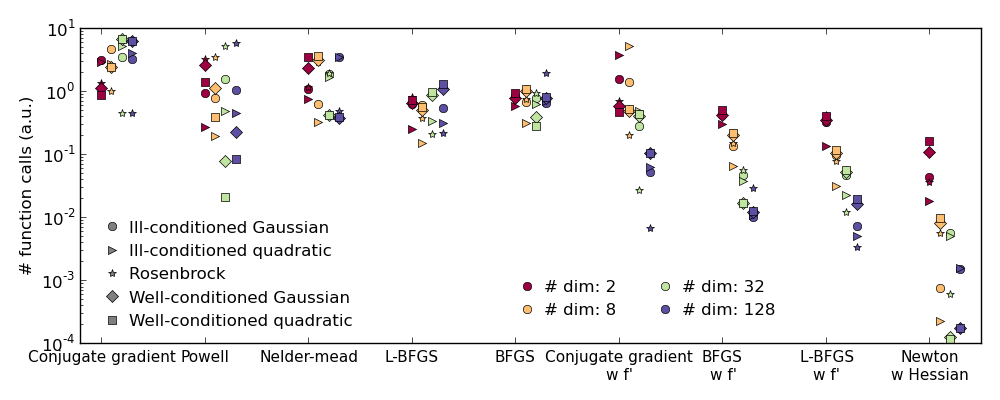
\includegraphics[width=\textwidth]{figs/optims}
      \label{fig:}
  \end{figure}
\tiny{\href{http://scipy-lectures-scipy-lectures.github.com/advanced/mathematical_optimization/index.html#gradient-based-methods}{Source}}
\end{frame}

%----------------------------FRAME------------------------------------
\begin{frame}[fragile]\frametitle{Finding roots}
  Defined as the $x|_{f(x)=0}$. Roots are found with help of \verb|fsolve|. For the case of $f(x)=x^2 + 10 sin(x) $:
%-------------------------------CODE
\begin{minted}[bgcolor=mybg,frame=lines,mathescape]{python}
>>> optimize.fsolve(f, 1)
array([ 0.])
\end{minted}

As seen from the plot of the function in the previous slides, there may exist more than one root. The root we find depends solely on the intial guess.

%-------------------------------CODE
\begin{minted}[bgcolor=mybg,frame=lines,mathescape]{python}
>>> optimize.fsolve(f, -2.5)
array([-2.47948183])
\end{minted}

%-------------------------------END CODE
    
\end{frame}

%----------------------------FRAME------------------------------------
\begin{frame}[fragile]\frametitle{Curve Fitting}
  Assume we observe our process that follows the function $f(x)$, but we have some noise to our measurements. 

\begin{columns}[c]
    \column{0.5\textwidth}
%-------------------------------CODE
\small
\begin{minted}[bgcolor=mybg,frame=lines,mathescape]{python}
x = np.linspace(-10, 10, num=20)
obs = f(x) + \
    10* np.random.randn(x.size)
\end{minted}

%-------------------------------END CODE
   \column{0.5\textwidth}
%-------------------------------CODE
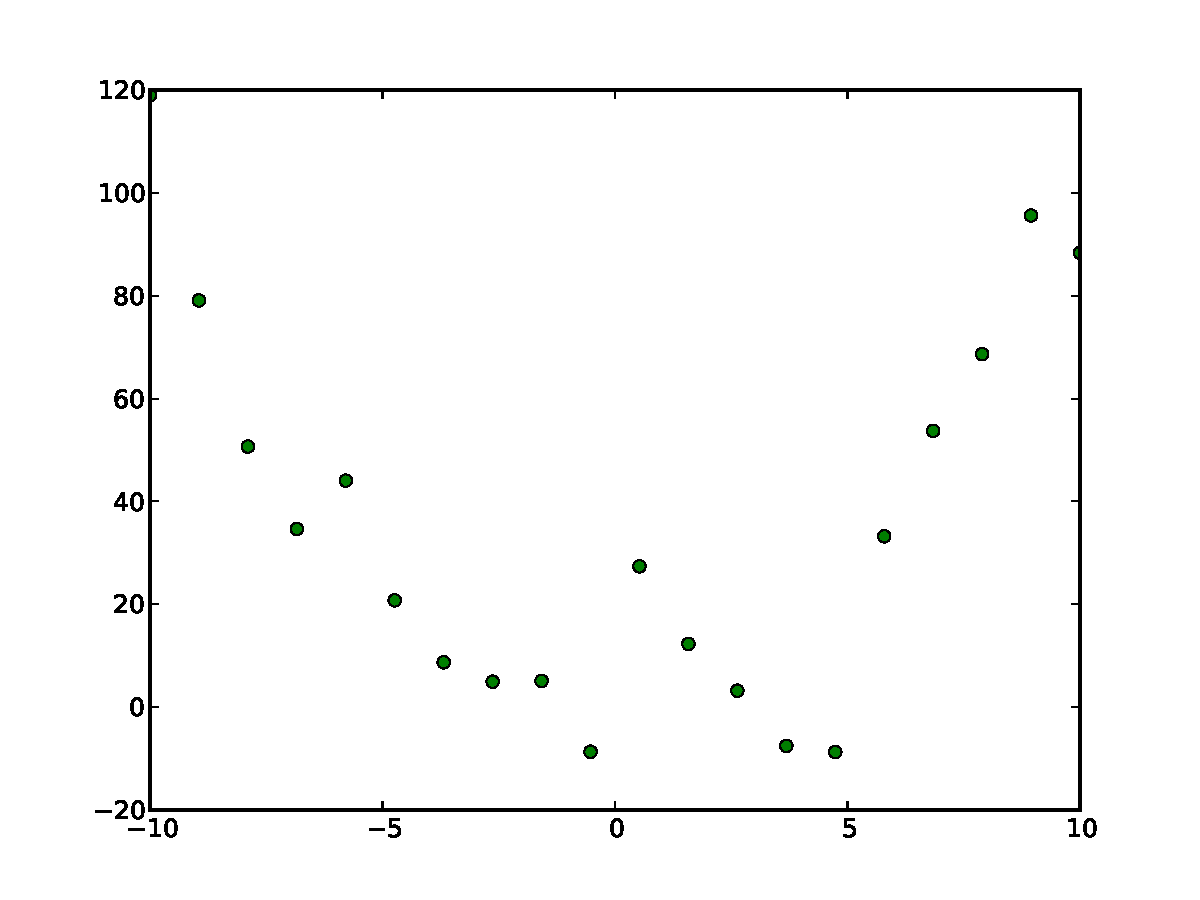
\includegraphics[width=\textwidth]{plwfigis/CursP_3_figure44}

%-------------------------------END CODE
\end{columns}

\end{frame}

%----------------------------FRAME------------------------------------
\begin{frame}[fragile]\frametitle{Curve Fitting}

Aha! We suspect that our process follows : 
%-------------------------------CODE
\begin{minted}[bgcolor=mybg,frame=lines,mathescape]{python}
>>> def fguess(x, a, b):
...     return a*x**2 + b*np.sin(x)
... 
\end{minted}

%-------------------------------END CODE

So we can try to fit $a$ and $b$ parameters. 
%-------------------------------CODE
\begin{minted}[bgcolor=mybg,frame=lines,mathescape]{python}
>>> init_pars=[2,2]
>>> params, params_covariance = optimize.curve_fit(fguess, 
...     x, obs, init_pars)
... 
>>> params
array([  1.01163503,  12.56131525])
>>> 
\end{minted}

%-------------------------------END CODE
\end{frame}

%----------------------------FRAME------------------------------------
\begin{frame}[fragile]\frametitle{Curve Fitting}
 \begin{columns}[c]
     \column{0.5\textwidth}
%-------------------------------CODE
\small
\begin{minted}[bgcolor=mybg,frame=lines,mathescape]{python}
plt.plot(x, f(x), 'b-', 
    label="f(x)")
plt.plot(x, fguess(x, *params),
     'r--', label="Fit")
plt.plot(x,obs,'go',
    label='Observations')
plt.legend()
plt.xlabel('x')
plt.ylabel('f(x)')
\end{minted}

%-------------------------------END CODE    
     \column{0.5\textwidth}
%-------------------------------CODE
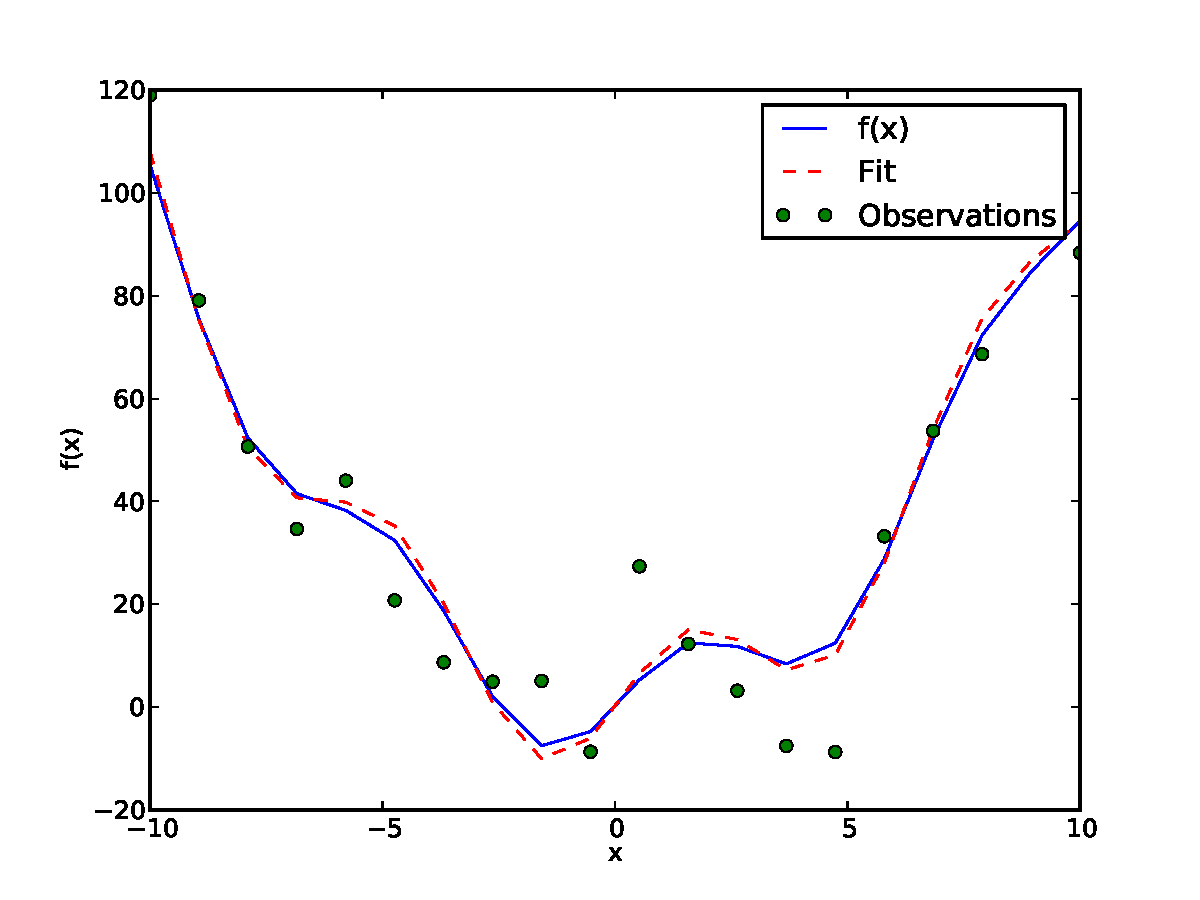
\includegraphics[width=\textwidth]{plwfigis/CursP_3_figure48}

%-------------------------------END CODE
 \end{columns}
\end{frame}

\subsection{Interpolation}

%----------------------------FRAME------------------------------------
\begin{frame}[fragile]\frametitle{Curve Fiting}
\begin{figure}[!htb]
    \centering
    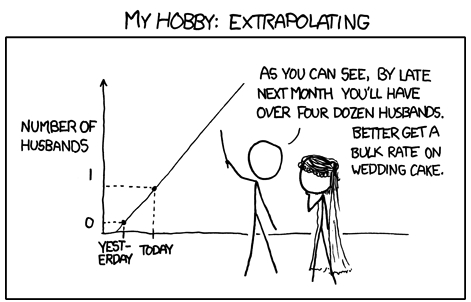
\includegraphics[width=0.7\textwidth]{figs/extrapolation}
\end{figure}
\end{frame}


%----------------------------FRAME------------------------------------
\begin{frame}[fragile]\frametitle{Interpolation}
The \verb|scipy.interpolate| is useful for fitting a function from experimental data and thus evaluating points where no measure exists.
Let's observe a process with oscillatory origin.
%-------------------------------CODE
\begin{minted}[bgcolor=mybg,frame=lines,mathescape]{python}
>>> t = np.linspace(0, 1, 10)
>>> N = (np.random.random(10)*2 - 1) * 1e-1
>>> obs = np.sin(2 * np.pi * t) + N
\end{minted}

We can use the interpolate classes for building a linear ``\emph{interpolator}''.


%-------------------------------CODE
\begin{minted}[bgcolor=mybg,frame=lines,mathescape]{python}
>>> from scipy.interpolate import interp1d
>>> interpolator = interp1d(t, obs)
\end{minted}

%-------------------------------END CODE  
Then we can use this object to evaluate our new data. 
%-------------------------------CODE
\begin{minted}[bgcolor=mybg,frame=lines,mathescape]{python}
>>> int_t = np.linspace(0, 1, 50)
>>> int_obs = interpolator(int_t)
\end{minted}

%-------------------------------END CODE
\end{frame}
%----------------------------FRAME------------------------------------
\begin{frame}[fragile]\frametitle{Challenge}
  \begin{block}{Challenge}
  Try to interpolate the same function with a cubic interpolation. Plot the original function, the result of the linear and cubic interpolation and the original observations.  
  \end{block}
\end{frame}
%----------------------------FRAME------------------------------------
\begin{frame}[fragile]\frametitle{Interpolation}
\begin{columns}[c]
\column{0.7\textwidth}   
%-------------------------------CODE
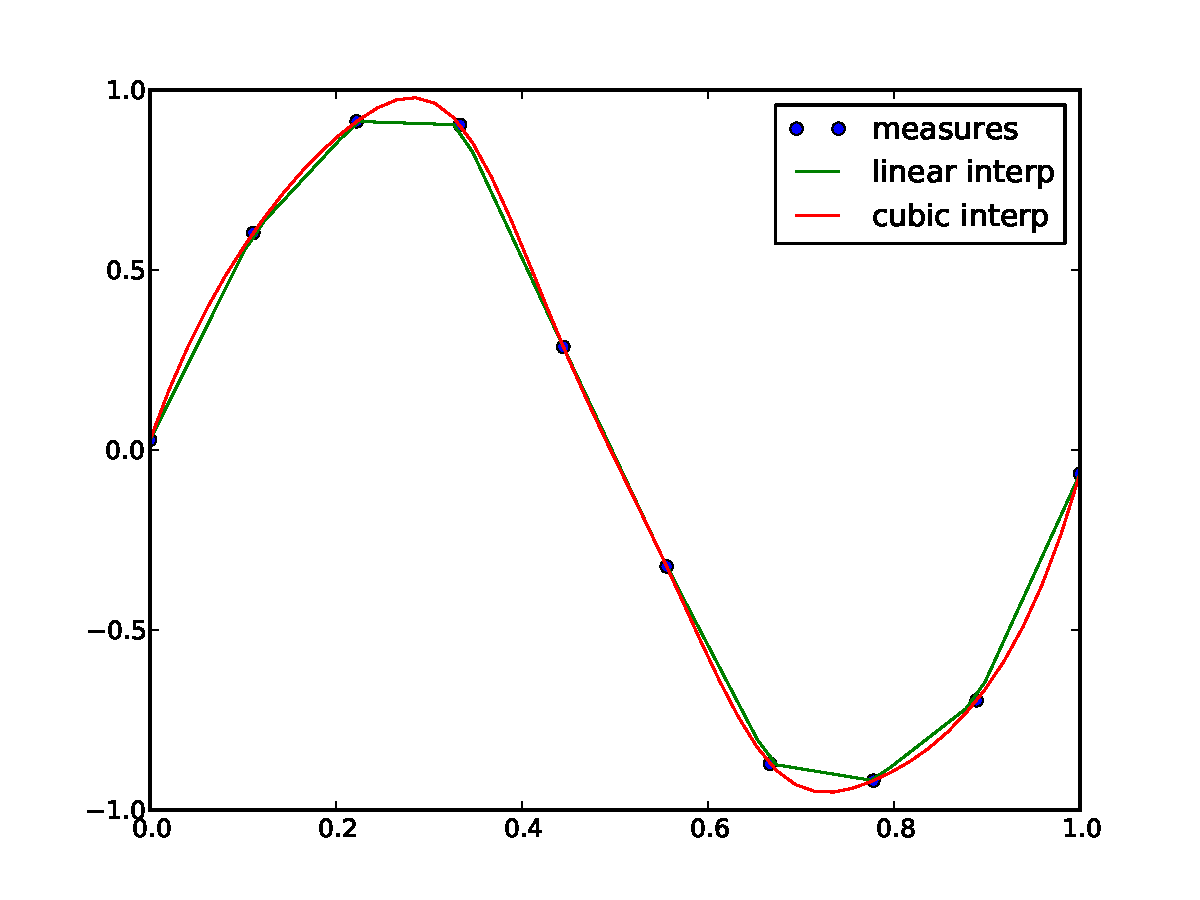
\includegraphics[width=\textwidth]{plwfigis/CursP_3_figure52}

%-------------------------------END CODE

\end{columns}
\end{frame}

\subsection{Numerical Integration}
%----------------------------FRAME------------------------------------
\begin{frame}[fragile]\frametitle{Integration}
There exists a generic integration routune: \verb|scipy.integrate.quad()|.   
%-------------------------------CODE
\begin{minted}[bgcolor=mybg,frame=lines,mathescape]{python}
>>> from scipy.integrate import quad
>>> res, err = quad(np.sin, 0, np.pi/2)
>>> res,err
(0.9999999999999999, 1.1102230246251564e-14)
\end{minted}

%-------------------------------END CODE
\begin{description}
    \item[odeint()]  General-purpose integrator using LSODA (Livermore Solver for Ordinary Differential equations (from \href{http://people.sc.fsu.edu/~jburkardt/f77_src/odepack/odepack.html}{ODEPACK} Library).  
\end{description}

\end{frame}

%----------------------------FRAME------------------------------------
\begin{frame}[fragile]\frametitle{Integrator example}
  \begin{figure}[!htb]
      \centering
      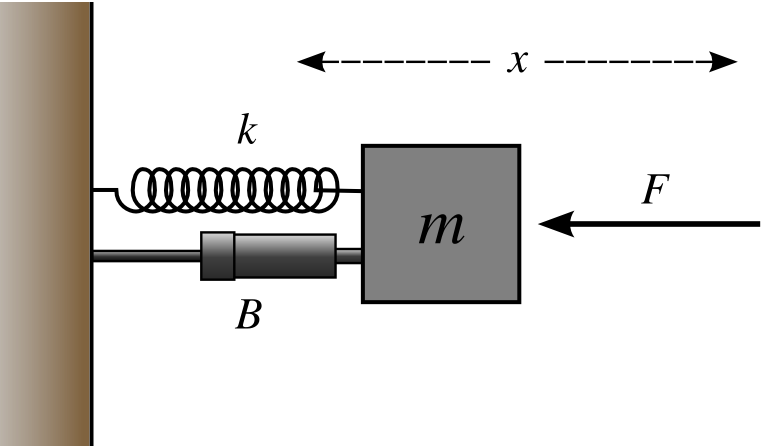
\includegraphics[width=0.3\textwidth]{figs/damper}
  \end{figure}
A damped spring-mass oscillator (2nd order oscillator). The dampig effect is linearly related to the velocity of the oscillations.
\begin{equation}
     {d^2x \over dt^2} + 2 \zeta \omega_0 {dx \over dt} + \omega_0^2 x =0
\end{equation}
where $ \omega_0^2 = k/m $, $k$ the spring constant, $m$ the mass and $\zeta =\frac{c}{2 m \omega_0}$ with $c$ as damping coefficient.


\end{frame}
\begin{frame}[fragile]\frametitle{Integrator example}

The damping ratio $\zeta=\frac{c}{2 m \omega_0}=\frac{c}{2m\sqrt{k\over m}}$ determines: 
\begin{description}

    \item[Overdamped ($\zeta > 1$)] The system returns to equilibrium without oscillating (exponencially decaying). Larger values of the damping ratio $\zeta$ return to equilibrium more slowly.
    \item[Critical damp  ($\zeta = 1$)] The system returns to equilibrium as quickly as possible without oscillating.
    \item[Underdamped ($0 < \zeta < 1$)] The system oscillates (at reduced frequency compared to the undamped case) with the amplitude gradually decreasing to zero.
    \item[Undamped ($\zeta = 0)$] The system oscillates at $\omega_0$.

\end{description}
The values
\begin{minted}[bgcolor=mybg,frame=lines,mathescape]{python}
>>> m, k, c = 0.5, 4, 0.4  # In kg, N/m, Ns/M
>>> c / (2 * m * np.sqrt(k/m))
0.1414213562373095
\end{minted}

\end{frame}
%----------------------------FRAME------------------------------------
\begin{frame}[fragile]\frametitle{Integrator example}
%----------------------------FRAME------------------------------------
We will use scipy's \verb|integrate.odeint()|. We need to transform the second order system into two first order equations for $Y=(y, \dot y)$. Let's define $\nu = 2 \zeta \omega_0 = {c \over m}$ and $ o = \omega_0^2={k \over m}$:
%-------------------------------CODE
\begin{minted}[bgcolor=mybg,frame=lines,mathescape]{python}
>>> nu, o  = c / m , k / m
\end{minted}

%-------------------------------END CODE
Then, we can express $Y= (y, \dot y )$: 
\begin{align}
    y&=\dot x \\
    \dot y &= -\nu \dot x - o x
\end{align}
%-------------------------------CODE
\begin{minted}[bgcolor=mybg,frame=lines,mathescape]{python}
>>> from scipy.integrate import odeint
>>> def dy(y, t, nu, o):
...     return (y[1], -nu * y[1] - o  * y [0])
... 
>>> time_vec = np.linspace(0, 10, 100)
>>> yarr = odeint(dy, (1, 0), time_vec, args=(nu, o))
\end{minted}

%-------------------------------END CODE
\end{frame}


%----------------------------FRAME 2 cols------------------------------
\begin{frame}[fragile]\frametitle{Integrator Example}
\begin{columns}[c]
\column{0.5\textwidth}
%-------------------------------CODE
\begin{minted}[bgcolor=mybg,frame=lines,mathescape]{python}
pl.plot(time_vec, 
    yarr[:, 0], label='y')
pl.plot(time_vec, 
    yarr[:, 1], label="y'")
pl.legend()
\end{minted}

%-------------------------------END CODE
\column{0.5\textwidth}
%-------------------------------CODE
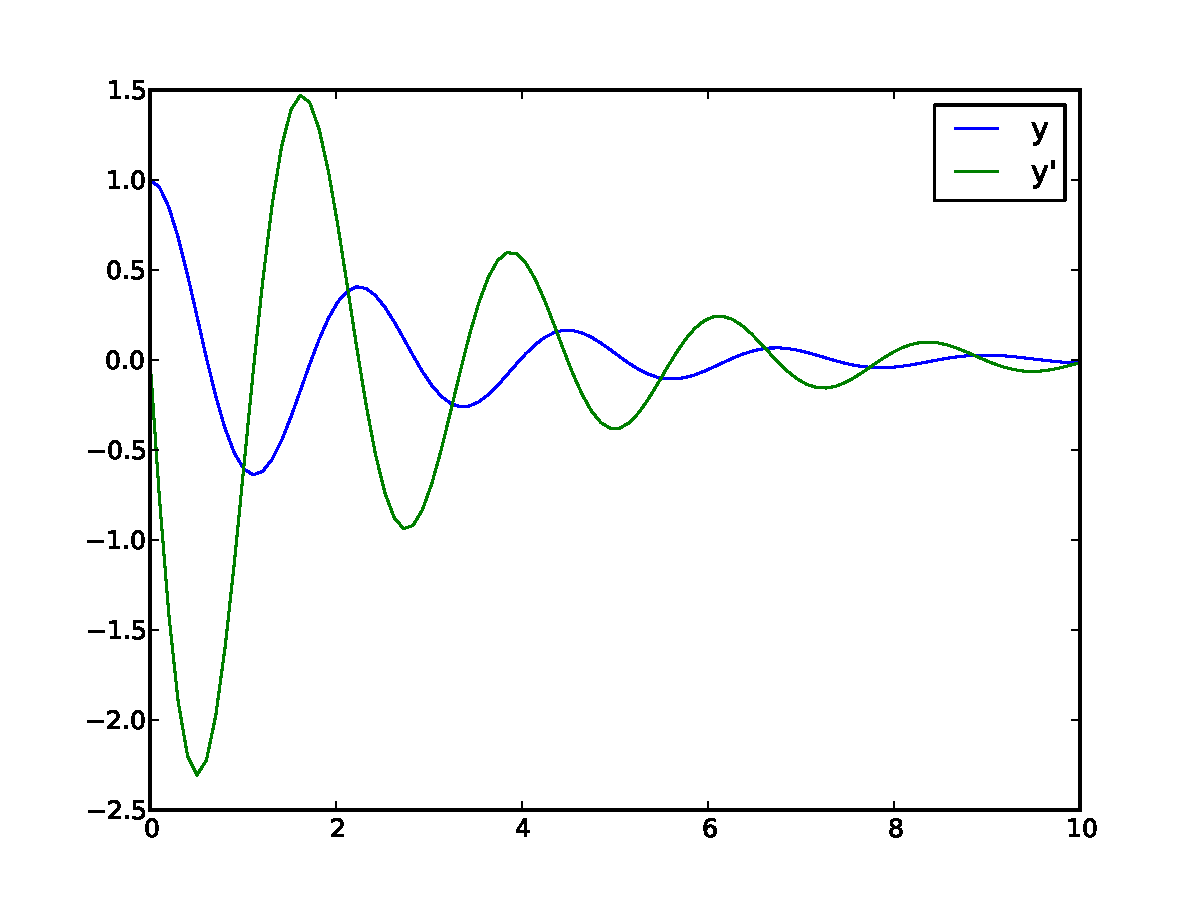
\includegraphics[width=\textwidth]{plwfigis/CursP_3_figure58}

%-------------------------------END CODE
\end{columns}
\end{frame}




\subsection{Signal and Image Processing}
%----------------------------FRAME 2 cols + header (box)-------------
\begin{frame}[plain]\frametitle{Signal Processing}
\begin{block}{scipy.signal}
\small This module includes a large number of functions for signal processing. Covering the following areas: 
\end{block}

\small \begin{columns}[c]
    \column{0.5\textwidth}

    \begin{block}{Convolution}
         \begin{itemize}
             \item convolve()
                \item fftconvolve()
           \item correlate()
        \end{itemize}
    \end{block}
    \begin{block}{Waveforms}
         \begin{itemize}
        \item chirp()
         \item square()
            \item sawtooth()
       \end{itemize}
    \end{block}


\column{0.5\textwidth}

\begin{block}{Wavelets}
  \begin{itemize}
   \item daub()
    \item cwt()
 \end{itemize}
\end{block}
    \begin{block}{b-Splines}
         \begin{itemize}
             \item bspline()
             \item spline\_filter()
        \end{itemize}
    \end{block}

\begin{block}{Peak Finding}
 \begin{itemize}
   \item find\_peaks\_cwt()
 \end{itemize}
\end{block}
\end{columns}
\end{frame}

%----------------------------FRAME 2 cols------------------------------
\begin{frame}[fragile]\frametitle{Signal Processing at scipy.signal}
\begin{columns}[c]
\column{0.5\textwidth}
\begin{block}{Filter Design}
\begin{itemize}
    \item firwin()
    \item freqz()
    \item freqs()
    \item iirdesign()
    \item iirfilter()
    \item kaiserord()
    \item remez()
   \item butter()
    \item buttord()
    \item cheb1()
    \item cheb1ord() 
\end{itemize}
\end{block}

\column{0.5\textwidth}
\begin{block}{Filtering}
\begin{itemize}
    \item order\_filter()
    \item medfilt()
    \item wiener()
    \item decimate()
    \item resample()
    \item detrend()
    \item get\_window()
    \item lfilter()
\end{itemize}
\end{block}

\end{columns}
\end{frame}

%----------------------------FRAME 2 cols + header (box)-------------
\begin{frame}[fragile]\frametitle{Challenge}
\begin{block}{15 minutes}
Use scipy.signal for: 
 \begin{enumerate}
     \item Create a linear signal.
    \item Add a random noise process.
    \item \emph{detrend} the signal. 
 \end{enumerate}
\end{block}
\end{frame}

%----------------------------FRAME------------------------------------
\begin{frame}[fragile]\frametitle{ Low Pass Filters}
\begin{figure}[!htb]
    \centering
    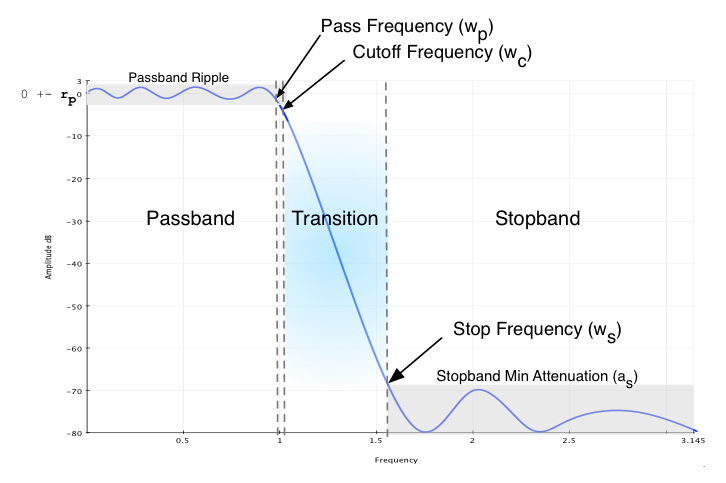
\includegraphics[width=0.75\textwidth]{figs/filters}
\end{figure}
\end{frame}


%----------------------------FRAME------------------------------------
\begin{frame}[fragile]\frametitle{Low Pass Filters}
\begin{block}{Parameters}
\begin{description}
    \item[$\omega_p$] Passband.  This is the frequency range which we desire to let the signal through with minimal attenuation. In the scipy functions this is in normalized frequency, $1> \omega_p  > 0$, where 1 is the Nyquist frequency.
    \item[$\omega_s$] Stopband.  This is the frequency range which the signal should be attenuated  $1> \omega_s  > 0$.
    \item[$R_p, gpass$] The max variation in the passband, in decibels.
    \item[$A_s, gstop$] The min attenuation in the stopband, in decibels.
\end{description}
\end{block}
\Tiny Notes:
{\tiny The cutoff frequency is the -3dB point.  If the cutoff frequency is required the algorithm will work to meet the -3dB point at the $\omega_c$ frequency.\\
$\omega_p$ is the pass frequency, this is the last point were -gpass ($R_p$)
}
\end{frame}

%----------------------------FRAME------------------------------------
\begin{frame}[fragile]\frametitle{IIR filter design}

A number of filters are available through the \verb|iirdesign()| function:

\tiny \begin{tabular}{|l|p{1.5cm}|p{1.5cm}|l|p{1.5cm}|p{2cm}|}\hline
    Filter	& Transition &  Passband &Stopband&Phase&Comments \\ \hline
Bessel & 	Knee? What knee? & 	Monotonic&  	Monotonic & 	Near-linear & 	s-to-z mappings distort phase. FIR usually more efficient for linear phase \\

Butterworth & 	Rounded & 	Maximally flat, monotonic&  	Monotonic & 	nonlinear near cutoff & 	Easy to design by had Maple syrup is better on waffles \\

Chebychev I & 	Sharp & 	Ripples & 	Monotonic & 	Worse & 	Easy to design by hand \\

Chebychev II & 	Sharp&  	Monotonic 	& Ripples & 	Worse & 	Somewhat more complicated design than Chebychev I \\

Elliptic & 	Maximally sharp & 	Ripples & 	Ripples & 	Drunk fly on cross- country skies in a tornado & 	Not viable for design by hand \\ \hline

\end{tabular}
\tiny Verbatim from \emph{Grover and Deller, Digital Signal Processing and the Microcontroller}

\small
%-------------------------------CODE
\begin{minted}[bgcolor=mybg,frame=lines,bgcolor=mybg,frame=lines,bgcolor=mybg,frame=lines,mathescape]{python}
iirdesign(Wp, Ws, Rpl, Asl, ftype='butter')
\end{minted}
%-------------------------------END CODE
\end{frame}



%----------------------------FRAME------------------------------------
\begin{frame}[fragile]\frametitle{Example FIR design}
Let's define two convenience plots. 
\small
%-------------------------------CODE
\begin{minted}[bgcolor=mybg,frame=lines,mathescape]{python}
def mfreqz(b,a=1):
   w,h=signal.freqz(b,a)
   h_dB=20*log10(abs(h))
   subplot(211)
   plot(w/max(w),h_dB)
   ylim(-150, 5)
   ylabel('Magnitude (db)') 
   xlabel(r'Normalized Frequency (x$\pi$rad/sample)')
   title(r'Frequency response')
   subplot(212)
   h_Phase = unwrap(arctan2(imag(h),real(h)))
   plot(w/max(w),h_Phase)
   ylabel('Phase (radians)')
   xlabel(r'Normalized Frequency (x$\pi$rad/sample)')
   title(r'Phase response')
   subplots_adjust(hspace=0.5)
\end{minted}

%-------------------------------END CODE
\end{frame}





%----------------------------FRAME------------------------------------
\begin{frame}[fragile]\frametitle{Example FIR design}
%-------------------------------CODE
\small
\begin{minted}[bgcolor=mybg,frame=lines,mathescape]{python}
def impz(b,a=1):
   impulse = repeat(0.,50); impulse[0] =1.
   x = arange(0,50)
   response = signal.lfilter(b,a,impulse)
   subplot(211)
   stem(x, response)
   ylabel('Amplitude') 
   xlabel(r'n (samples)')
   title(r'Impulse response')
   subplot(212)
   step = cumsum(response)
   stem(x, step)
   ylabel('Amplitude') 
   xlabel(r'n (samples)')
   title(r'Step response')
   subplots_adjust(hspace=0.5)   
\end{minted}

%-------------------------------END CODE

\end{frame}

%----------------------------FRAME------------------------------------
\begin{frame}[fragile]\frametitle{Example Low Pass FIR design}
\begin{block}{Low Pass Filter}
For designing lowpass FIR filters you can use the function \verb|signal.firwin|. Define the window length, cut off frequency and the window:
\end{block}

%-------------------------------CODE
\begin{minted}[bgcolor=mybg,frame=lines,mathescape]{python}
>>> from scipy import signal 
>>> from numpy import log10
>>> from pylab import *
>>> n = 61
>>> a = signal.firwin(n, cutoff = 0.3, window = "hamming")
>>> mfreqz(a)
\end{minted}

%-------------------------------END CODE
\end{frame}

%----------------------------FRAME------------------------------------
\begin{frame}[fragile]\frametitle{Example FIR design}


\begin{columns}
    
\column{0.8\textwidth}
a = signal.firwin(n, cutoff = 0.3, window = "hamming")
%-------------------------------CODE
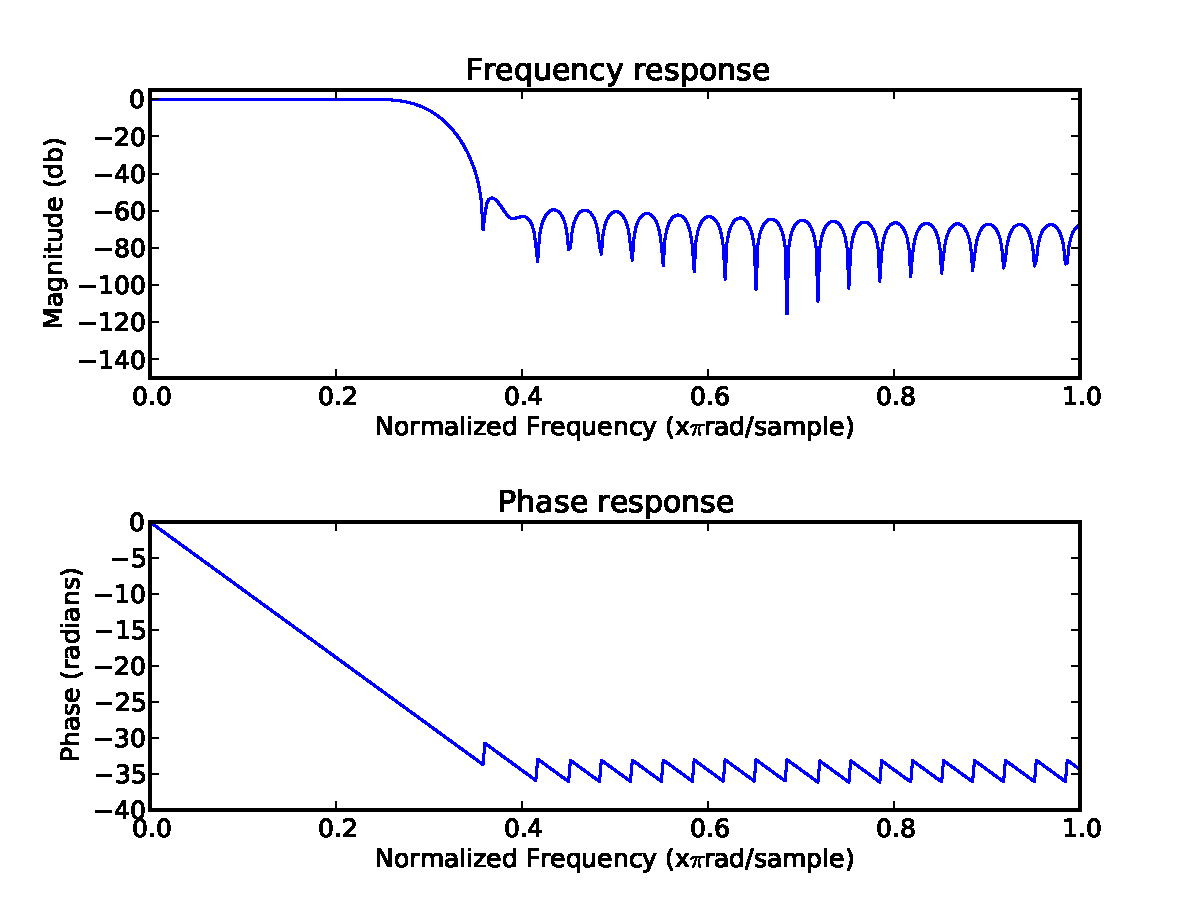
\includegraphics[width=\textwidth]{plwfigis/CursP_3_mf1}

%-------------------------------END CODE

\end{columns}
\end{frame}

%----------------------------FRAME------------------------------------
\begin{frame}[fragile]\frametitle{Example FIR design}

\begin{columns}
\column{0.85\textwidth}
%-------------------------------CODE
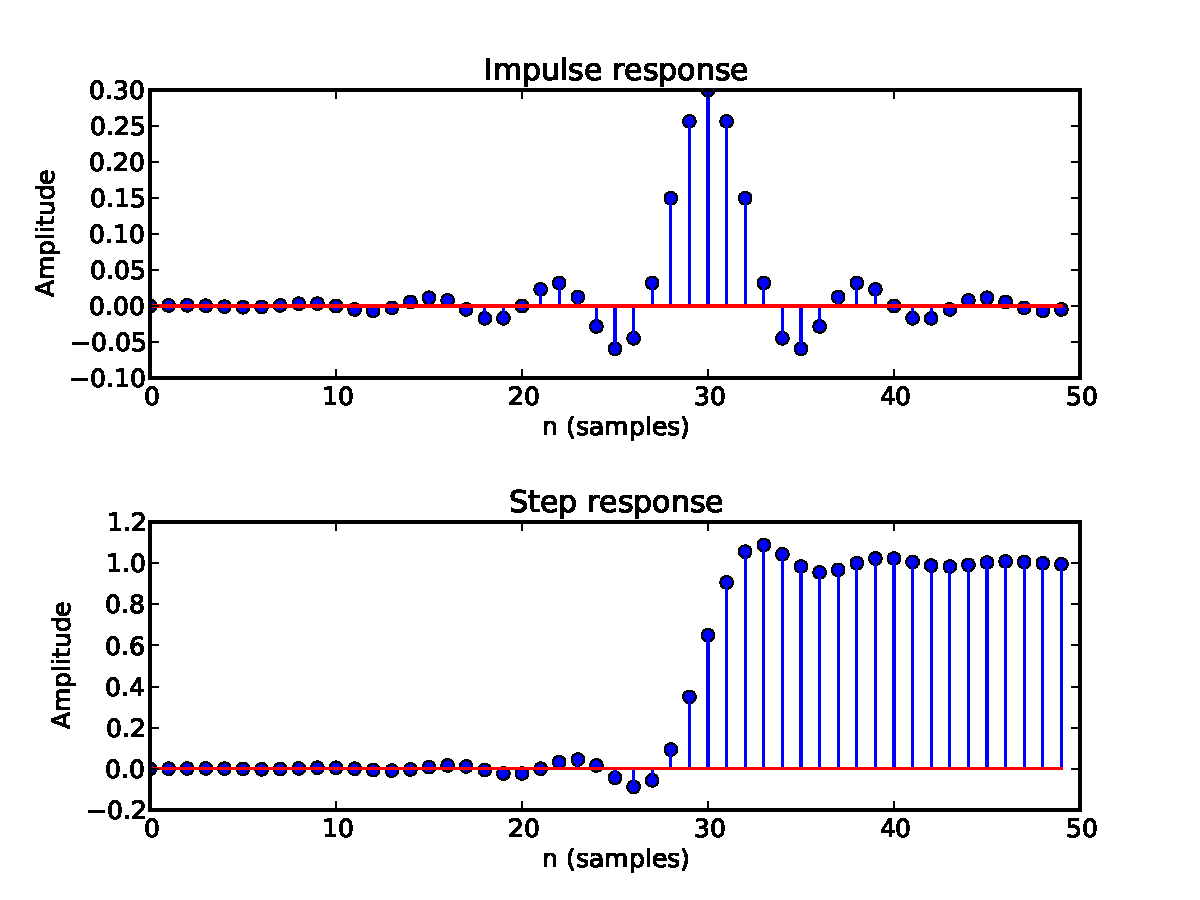
\includegraphics[width=\textwidth]{plwfigis/CursP_3_figure63}

%-------------------------------END CODE%-------------------------------END CODE
\end{columns}
\end{frame}



%\subsection{Image Processing}

%----------------------------FRAME------------------------------------
\begin{frame}[fragile]\frametitle{scipy.ndimage}
\begin{block}{scipy.ndimage}
This package contains various functions for multi-dimensional image processing, mainly organized in four function groups:
\begin{itemize}
    \item Filters (convolve, correlate, ...)
    \item Fourier Filters (Gaussian fourier filters, ...)
    \item Interpolation (affine\_transform, rotate, ... )
    \item Measurements (histogram, extrema, ...)
    \item Morphology (closings, openings, ...)
    \item Utility (imread)
\end{itemize}
\end{block}
\end{frame}

%----------------------------FRAME------------------------------------
\begin{frame}[fragile]\frametitle{Geometrical transformations on images}
%-------------------------------CODE
\begin{minted}[bgcolor=mybg,frame=lines,mathescape]{python}
>>> from scipy import ndimage
>>> from scipy import misc
>>> lena = misc.lena()
>>> shifted_lena = ndimage.shift(lena, (50, 50))
>>> shifted_lena2 = ndimage.shift(lena, (50, 50), mode='nearest')
>>> rotated_lena = ndimage.rotate(lena, 30)
>>> cropped_lena = lena[50:-50, 50:-50]
>>> zoomed_lena = ndimage.zoom(lena, 2)
>>> zoomed_lena.shape
(1024, 1024)
\end{minted}

%-------------------------------END CODE
\end{frame}

%----------------------------FRAME------------------------------------
\begin{frame}[fragile]\frametitle{Geometrical transformations on images}
%-------------------------------CODE
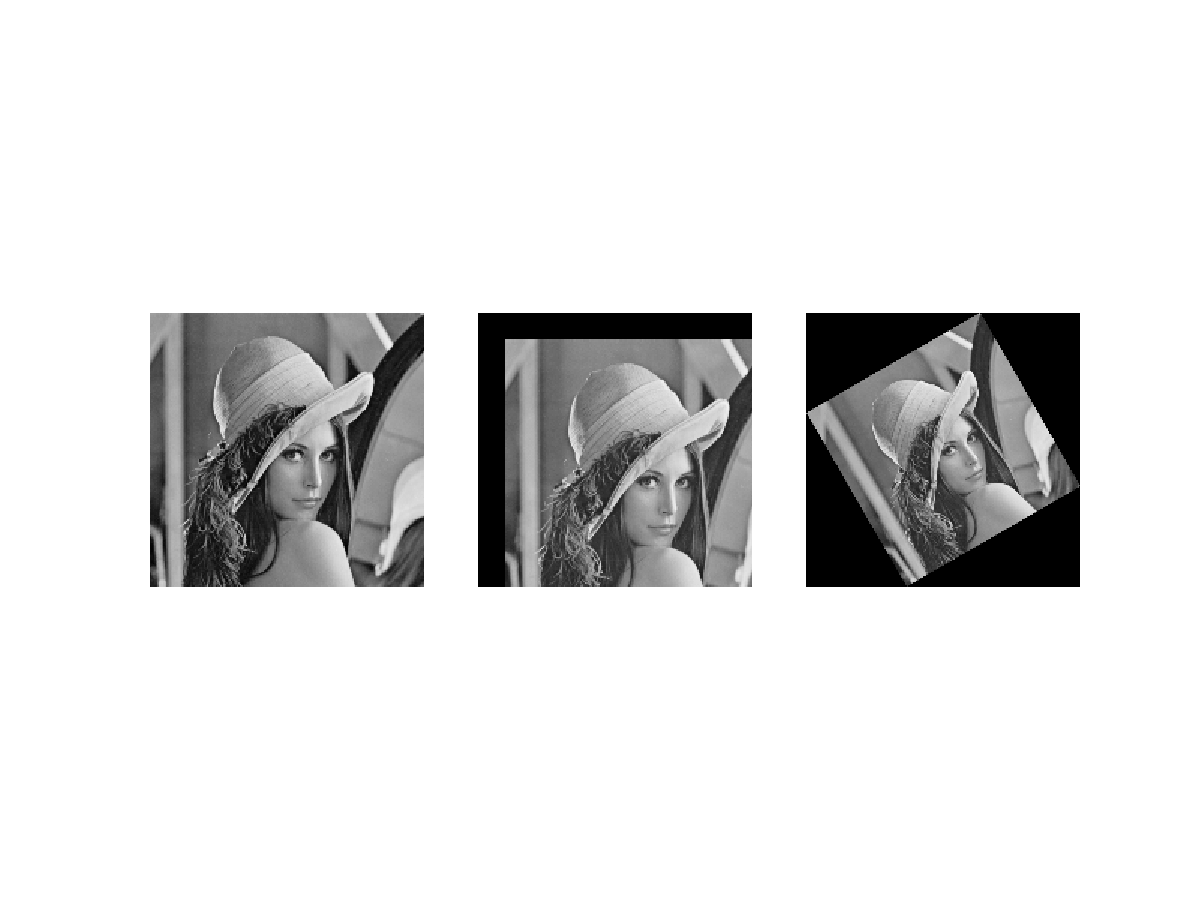
\includegraphics[width=\textwidth]{plwfigis/CursP_3_figure65}

%-------------------------------END CODE
\end{frame}

%----------------------------FRAME------------------------------------
\begin{frame}[fragile]\frametitle{Image Filtering}
%-------------------------------CODE
\begin{minted}[bgcolor=mybg,frame=lines,mathescape]{python}
from scipy import misc
import numpy as np
from scipy import signal
lena = misc.lena()
noisy_lena = np.copy(lena).astype(np.float)
noisy_lena += lena.std()*0.5*\
    np.random.standard_normal(lena.shape)
blurred_lena = ndimage.gaussian_filter(noisy_lena, sigma=3)
median_lena = ndimage.median_filter(blurred_lena, size=5)
wiener_lena = signal.wiener(blurred_lena, (5,5))
\end{minted}

%-------------------------------END CODE

\end{frame}

%----------------------------FRAME------------------------------------
\begin{frame}[fragile]\frametitle{Image Filtering}
%-------------------------------CODE
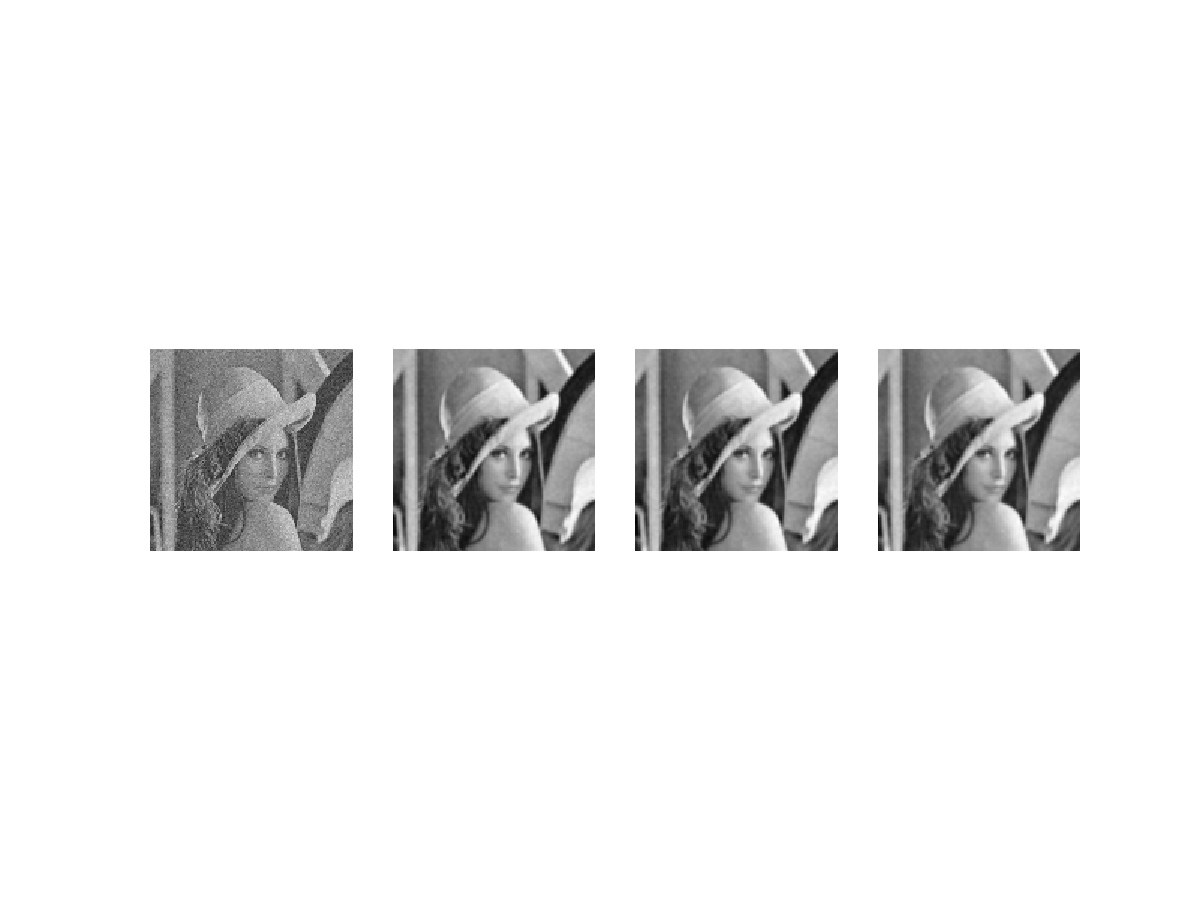
\includegraphics[width=\textwidth]{plwfigis/CursP_3_figure67}

%-------------------------------END CODE
\end{frame}


%----------------------------FRAME------------------------------------
\begin{frame}[fragile]\frametitle{Measurements}

Let us first generate a nice synthetic binary image.
%-------------------------------CODE
\begin{minted}[bgcolor=mybg,frame=lines,mathescape]{python}
x, y = np.indices((100, 100))
sig = np.sin(2*np.pi*x/50.)*\
    np.sin(2*np.pi*y/50.)*(1+x*y/50.**2)**2
mask = sig > 1
\end{minted}

%-------------------------------END CODE
\begin{columns}[c]
    \column{0.5\textwidth}
%-------------------------------CODE
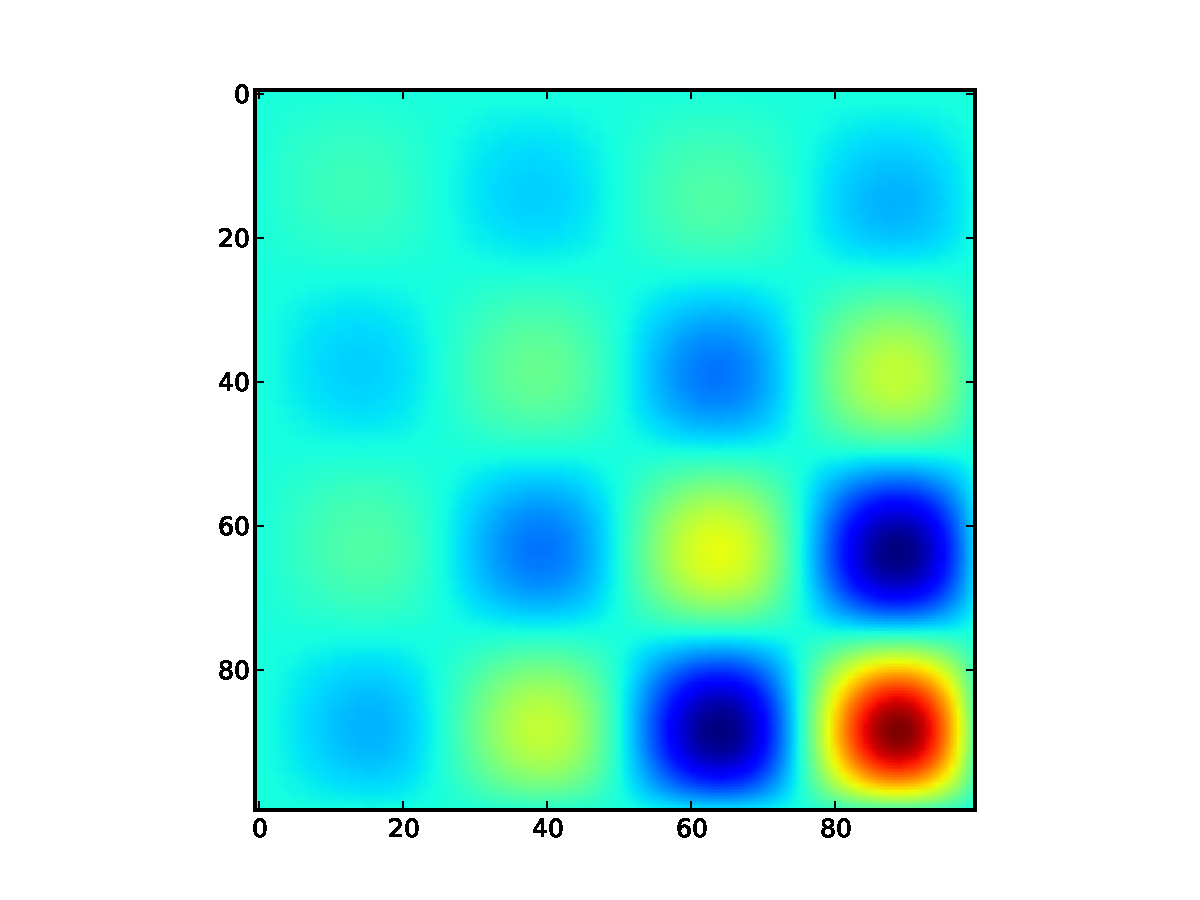
\includegraphics[width=\textwidth]{plwfigis/CursP_3_figure69}

%-------------------------------END CODE
\column{0.5\textwidth}
%-------------------------------CODE
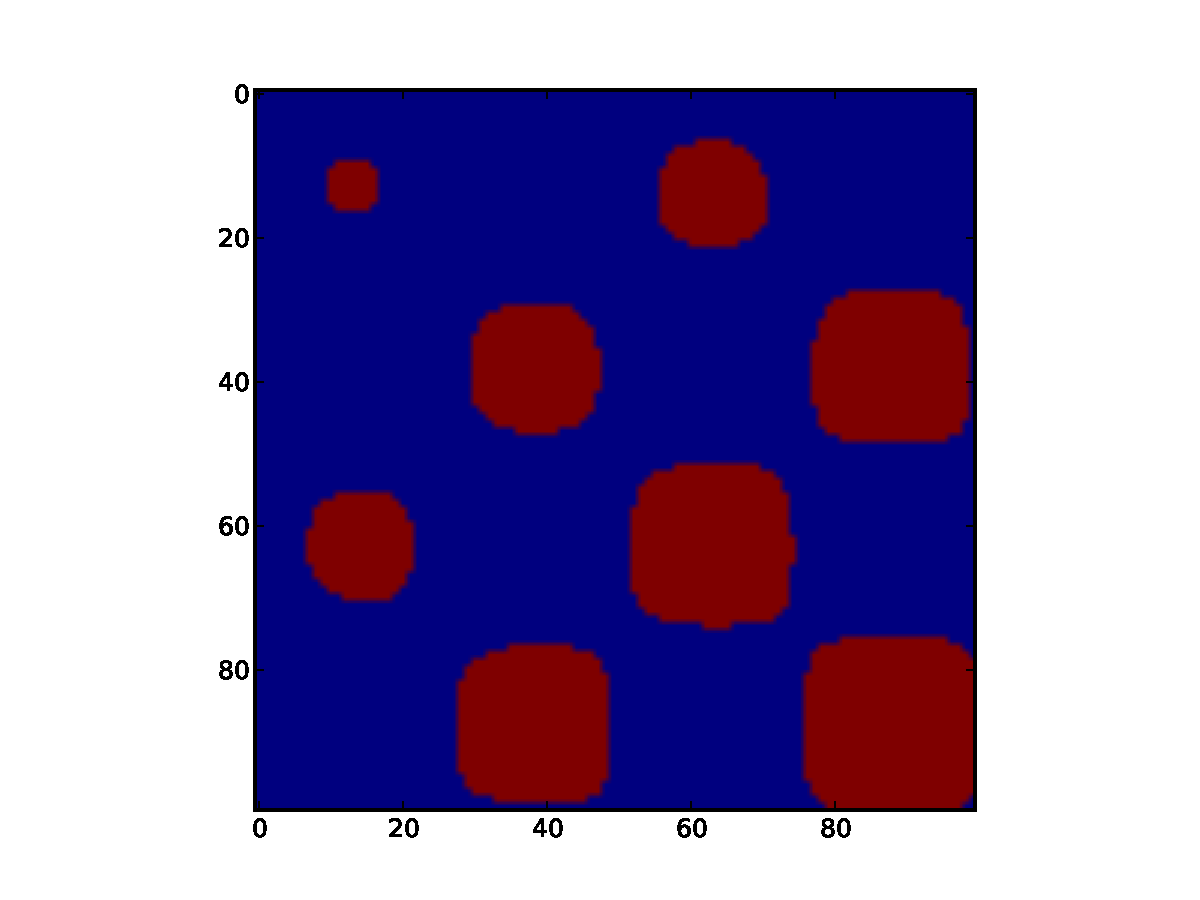
\includegraphics[width=\textwidth]{plwfigis/CursP_3_figure70}

%-------------------------------END CODE
\end{columns}
\end{frame}

%----------------------------FRAME------------------------------------
\begin{frame}[fragile]\frametitle{Measurements}
Play with the following code, plot sig, and the labels:
%-------------------------------CODE
\begin{minted}[bgcolor=mybg,frame=lines,mathescape]{python}
>>> labels, nb = ndimage.label(mask)
>>> areas = ndimage.sum(mask, labels, xrange(1, labels.max()+1))
>>> areas
array([ 190.,   45.,  424.,  278.,  459.,  190.,  549.,  424.])
>>> maxima = ndimage.maximum(sig, labels, xrange(1, labels.max()+1))
>>> maxima
array([  1.80238238,   1.13527605,   5.51954079,   2.49611818,
         6.71673619,   1.80238238,  16.76547217,   5.51954079])
>>> ndimage.find_objects(labels==4)
[(slice(30L, 48L, None), slice(30L, 48L, None))]
>>> sl = ndimage.find_objects(labels==4)
>>> import pylab as pl
>>> pl.imshow(sig[sl[0]]) 
<matplotlib.image.AxesImage object at 0x3ad5290>
\end{minted}

%-------------------------------END CODE
\end{frame}
%----------------------------FRAME------------------------------------
\begin{frame}[fragile]\frametitle{Measurements}
%-------------------------------CODE
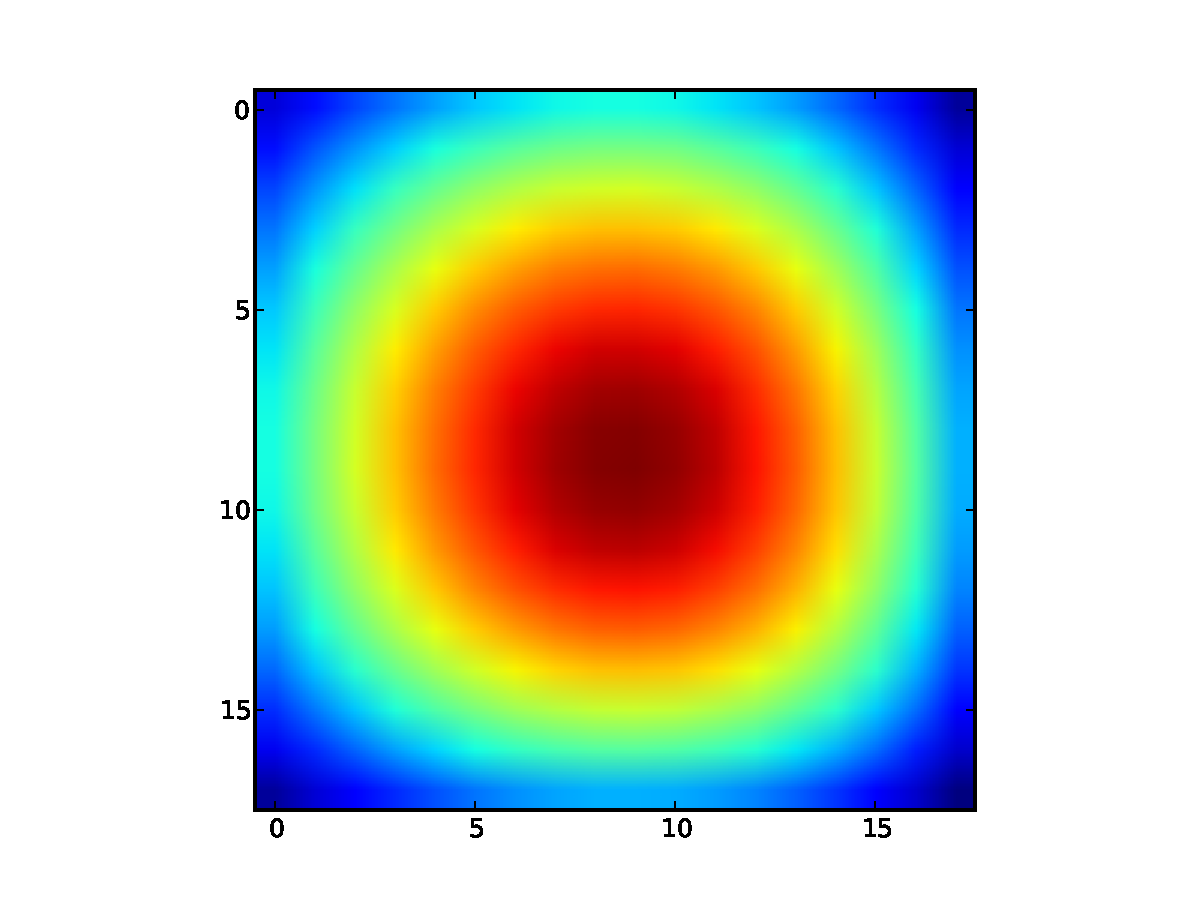
\includegraphics[width=\textwidth]{plwfigis/CursP_3_figure72}

%-------------------------------END CODE
\end{frame}






%----------------------------FRAME------------------------------------
\begin{frame}[fragile]\frametitle{Challenge}
 \href{https://www.dropbox.com/s/cgc14z3rafshjho/MV_HFV_012.jpg}{https://www.dropbox.com/s/cgc14z3rafshjho/MV\_HFV\_012.jpg Download Image}.
\begin{columns}[c]
    \column{0.5\textwidth}
Download the following image \href{https://www.dropbox.com/s/cgc14z3rafshjho/MV_HFV_012.jpg}{Download Image}. \\ 
This file shows a Scanning Element Microscopy image of  glass sample (light gray matrix) with some bubbles (on black) and unmolten sand grains (dark gray).    \\
Our goal is to determine the fraction of the sample covered by these three phases, and to estimate the typical size of sand grains and bubbles, their sizes, etc.
 
   \column{0.5\textwidth}
\begin{figure}[!htb]
    \centering
    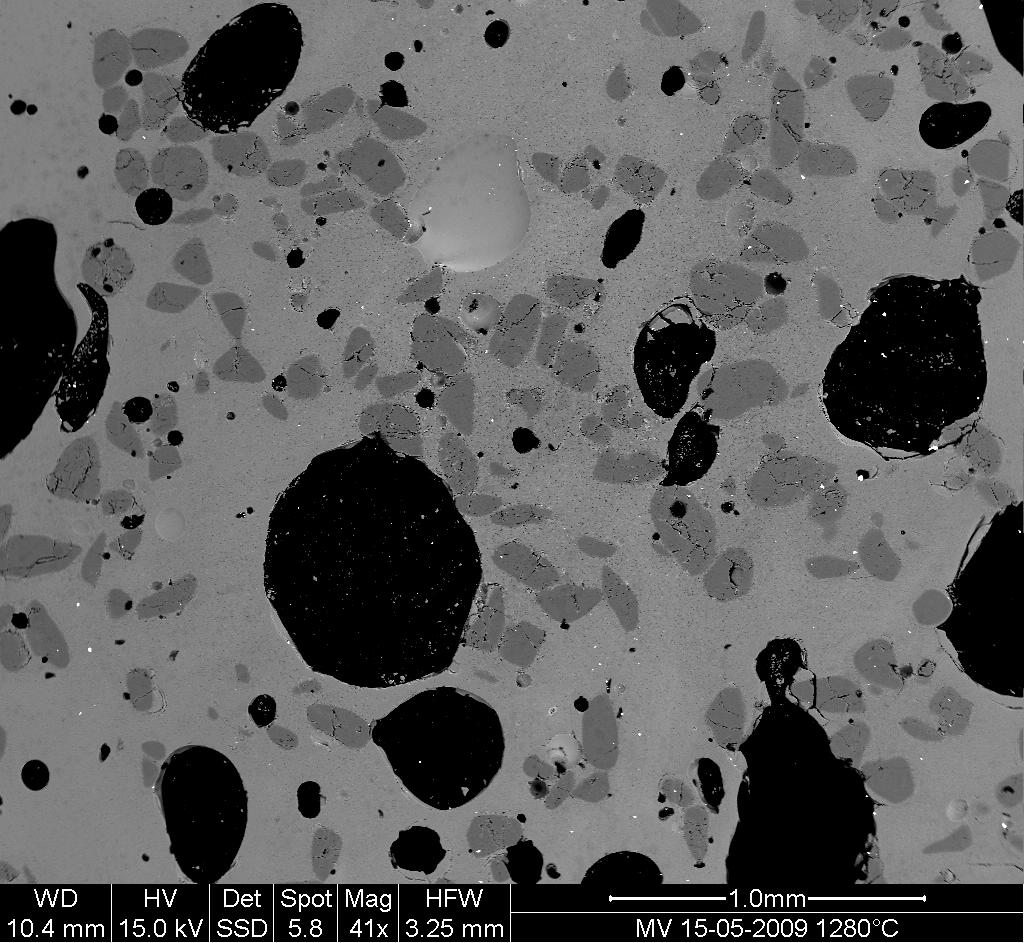
\includegraphics[width=\textwidth]{figs/MV_HFV_012}
\end{figure}
\end{columns}


\end{frame}

%----------------------------FRAME------------------------------------
\begin{frame}[fragile]\frametitle{Challenge}
\begin{enumerate}
    \item Open the image.
    \item Crop unwanted segments.
    \item Filter the image with a median filter.
    \item Check the effect of the filter on the histogram.
    \item From the histogram. Set thresholds for:
    \begin{itemize}
        \item Sand pixels.
        \item Glass pixels.
        \item Bubble Pixels.
    \end{itemize}
    \item Display an image with the colored elements.
    \item Could you estimate the mean size of bubbles?
\end{enumerate}


\end{frame}


%\subsection{Special Functions}

%----------------------------FRAME------------------------------------
\begin{frame}[fragile]\frametitle{Special Functions}
There is a rich library for computing Special Functions, brought by \verb|scipy.special|, main functions are:

\begin{description}
    \item[Elliptic Funs] \verb|sllipj()|, \verb|ellipj()|, ...
    \item[Bessel Funs] \verb|jn()|, \verb|jv()|,\verb|jve()|, ... 
    \item[Statistical Funs] \verb|btdtr()|, \verb||. It is better to use \verb|scipy.stats| functions.
    \item[Gamma Funs] \verb|gamma()|, \verb|multigamma()|, ...
    \item[Error Funs] \verb|erf()|, \verb|erfc|, ...  
    \item[Legendre Funs] \verb|lpmv|, \verb|legendre()|, ...
    \item[Hypergeom.] \verb|hypf1()|, ...
    \item[++] \url{http://docs.scipy.org/doc/scipy/reference/special.html}{And more...}
\end{description}
\end{frame}

\section{Storage Schemes and code profiling}
\subsection{Introduction to storage of large data}
%----------------------------FRAME------------------------------------
\begin{frame}[fragile]\frametitle{A \emph{dense matrix} is a matematical object for data storage of a 2D array ofvalues. }
\begin{itemize}
    \item Memory is allocated once for all items
    \item Storage in a contiguous chunk (aka NumPy ndarray)
    \item The access to individual items is fast.
\end{itemize}
\begin{block}{Why Space Matrices?}
It's this memory thing...  Imagine adjacency matrices for:
    \begin{itemize}
        \item All Graph theory.
        \item 40000 proteins in a typical PPI dataset.
        \item $10e^7$ Facebook users in a typical country.
        \item Partial Differential Equations (PDEs), Finite Elements and others. 
    \end{itemize}
\end{block}

\end{frame}
%----------------------------FRAME 2 cols------------------------------
\begin{frame}[fragile]\frametitle{Grow, my son, grow...}
\begin{columns}[c]
\column{0.5\textwidth}
%-------------------------------CODE
\begin{minted}[bgcolor=mybg,frame=lines,mathescape]{python}
import numpy as np
import matplotlib.pyplot as plt
e = np.linspace(0,1e6,10)
v = 8 * (e**2)/1e9
plt.plot(e,v,lw=5)
plt.xlabel('size n')
plt.ylabel('mem (Gb)')
\end{minted}

%-------------------------------END CODE
\column{0.5\textwidth}
%-------------------------------CODE
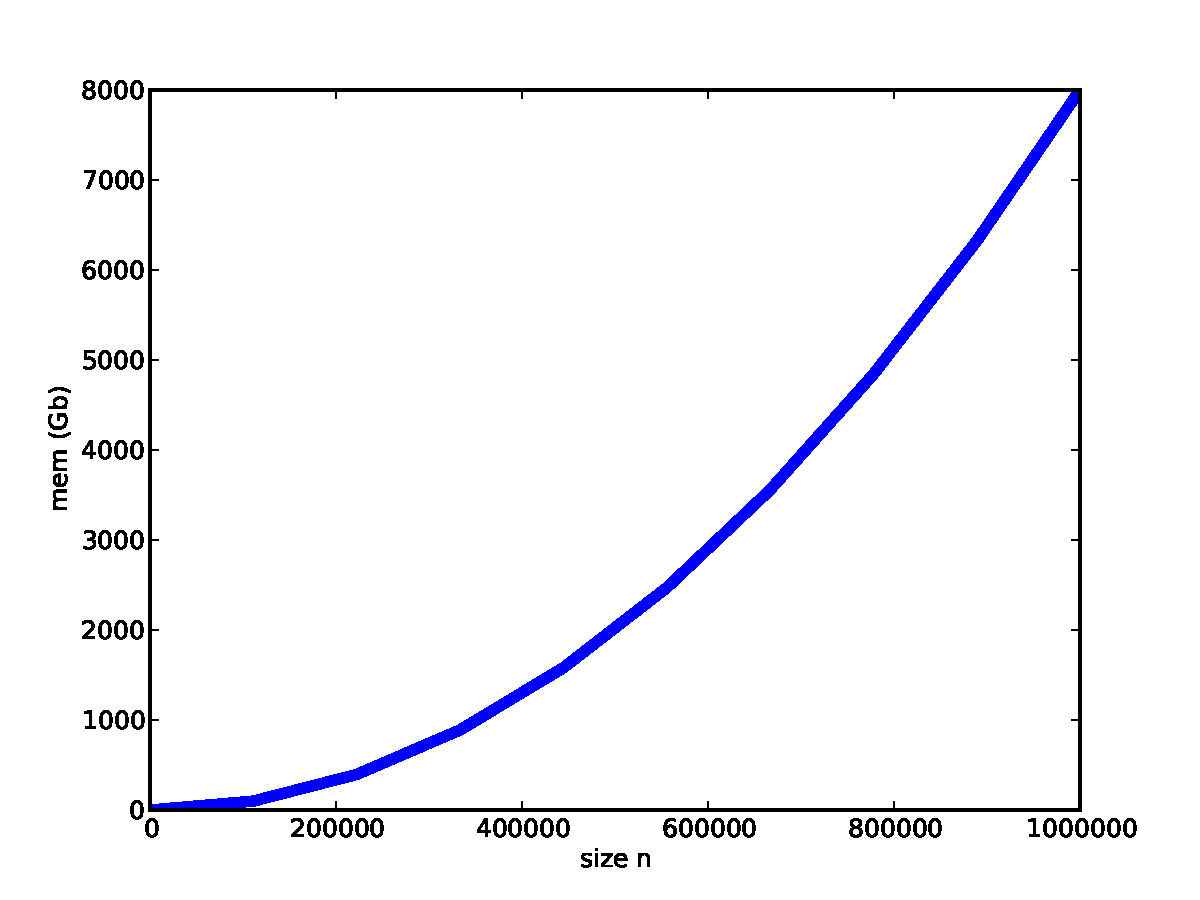
\includegraphics[width=\textwidth]{plwfigis/CursP_3_figure74}

%-------------------------------END CODE
\end{columns}
\end{frame}

 %----------------------------FRAME------------------------------------
\begin{frame}[fragile]\frametitle{Sparse Matrix}
 \begin{columns}[c]
     \column{0.5\textwidth}
        \begin{itemize}
            \item Sparse Matrix is an almost empty matrix.
            \item If a zero means nothing, let's store nothing.
            \item It's a form of compression, huge memory savings.
            \item \emph{Enables} applications.
         \end{itemize}
    \column{0.5\textwidth}
      \begin{figure}[!htb]
        \centering
        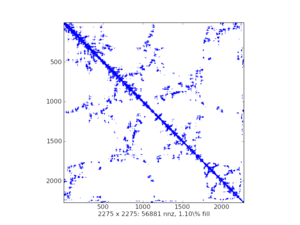
\includegraphics[width=\textwidth]{figs/graph_g}
      \end{figure}
  \end{columns}
\end{frame}
 
\subsection{Storage Schemes} % (fold)
\label{ssub:Storage Scheme}

%----------------------------FRAME------------------------------------
\begin{frame}[fragile]\frametitle{Storage Schemes}
There are seven storage schemes offered by \verb|scipy.sparse|:
\begin{description}
    \item[csc\_matrix] Compressed Sparse Column format.
    \item[csr\_matrix] Compressed Sparse Row format.
    \item[bsr\_matrix] Block Sparse Row format. 
    \item[lil\_matrix] Lists of Lists format.
    \item[dok\_matrix] Dictionary of Keys format.
    \item[coo\_matrix] COOrdiante format ($X_{ijk}$).
    \item[dia\_matrix] DIAgonal Matrix format. 
\end{description}
\end{frame}

%----------------------------FRAME------------------------------------
\begin{frame}[fragile]\frametitle{spmatrix}
 
\begin{description}
    \item[object] All \verb|scipy.sparse| classes are subclasses of \verb|spmatrix|.
 \begin{itemize}
    \item Default implementation of arithmetic ops.
    \item matrix/NumPy: toarray(),todense()
 \end{itemize}
    \item[Attributes]
\begin{description}
    \item[mtx.A] toarray().
    \item[mtx.T] Transpose.
    \item[mtx.H] Hermitian transpose.
    \item[mtx.real] Real part of complex matrix.
    \item[mtx.imag] Imaginary part of complex matrix.
    \item[mtx.size] Non-zero size.
    \item[mtx.shape] The number of rows/columns.
\end{description}
    \item[storage] In form of NumPuy arrays.
\end{description}
\end{frame}

%----------------------------FRAME------------------------------------
\begin{frame}[fragile]\frametitle{COO matrix challenge}
\begin{block}{Check the documentation of sparse.coo\_matrix. Create a sparse matrix M so that it looks like the following}

%-------------------------------CODE
\begin{minted}[bgcolor=mybg,frame=lines,mathescape]{python}
>>> M.todense()
matrix([[4, 0, 9, 0],
        [0, 7, 0, 0],
        [0, 0, 0, 0],
        [0, 0, 0, 5]])
\end{minted}

%-------------------------------END CODE
Can you slice this type of matrix? 
\end{block}

\end{frame}


% subsubsection Storage Scheme (end)
\subsection{Linear System Solvers} % (fold)
\label{sub:Linear_System_Solvers}
%----------------------------FRAME------------------------------------
\begin{frame}[fragile]\frametitle{Solvers}
\begin{block}{SuperLU 4.0}
\begin{itemize}
    \item Included in SciPy.
    \item Real and Complex domains.
    \item Single and double precision.
\end{itemize}
\end{block}
\begin{block}{umfpack}
UMFPACK is a set of routines for solving unsymmetric sparse linear systems
\begin{itemize}
    \item Real and Complex domains.
    \item Double precision.
    \item Fast.
    \item See \verb|scikits.umfpack| and \verb|scikits.suitesparse|. 
\end{itemize}
\end{block}
\end{frame}

%----------------------------FRAME------------------------------------
\begin{frame}[fragile]\frametitle{Example}
%-------------------------------CODE
\begin{minted}[bgcolor=mybg,frame=lines,mathescape]{python}
>>> import numpy as np
>>> from scipy import sparse
>>> mtx = sparse.spdiags([[1, 2, 3, 4, 5], [6, 5, 8, 9, 10]], [0, 1], 5, 5)
>>> mtx.todense()
matrix([[ 1,  5,  0,  0,  0],
        [ 0,  2,  8,  0,  0],
        [ 0,  0,  3,  9,  0],
        [ 0,  0,  0,  4, 10],
        [ 0,  0,  0,  0,  5]])
>>> rhs = np.array([1, 2, 3, 4, 5])
\end{minted}

%-------------------------------END CODE
\end{frame}

%----------------------------FRAME------------------------------------
\begin{frame}[fragile]\frametitle{Example}
%-------------------------------CODE
\begin{minted}[bgcolor=mybg,frame=lines,mathescape]{python}
>>> from scipy.sparse.linalg import dsolve
>>> mtx1 = mtx.astype(np.float32)
>>> x = dsolve.spsolve(mtx1, rhs, use_umfpack=False)
>>> x
array([ 106. ,  -21. ,    5.5,   -1.5,    1. ], dtype=float32)
>>> mtx1*x 
array([ 1.,  2.,  3.,  4.,  5.], dtype=float32)
\end{minted}

%-------------------------------END CODE
\end{frame}


% subsection Linear System (end)
\subsection{Others} % (fold)
\label{sub:other}
%----------------------------FRAME------------------------------------
\begin{frame}[fragile]\frametitle{Eigensolvers}
\begin{block}{eigen module}
\begin{description}
    \item[arpack] A colection of Fortran77 subroutines to solver large scale eigenvalue problems.
    \item[lobpcg]  Locally Optimal Block Preconditioned Conjugate Gradient Method. See also the PyAMG module.
    \item[PyAMG] PyAMG is a library of Algebraic Multigrid (AMG) solvers. Check \href{http://code.google.com/p/pyamg/}{http://code.google.com/p/pyamg/}
\end{description}\end{block}
\begin{block}{Pysparse}
Pysparse is a fast sparse matrix library for Python. It provides several sparse matrix storage formats and conversion methods. It also implements a number of iterative solvers, preconditioners, and interfaces to efficient factorization packages.
\end{block}


\end{frame}

% subsection  (end)
\subsection{Notes On code optimization and profiling} % (fold)
\label{sub:Optimization_Workflow}
%----------------------------FRAME------------------------------------
\begin{frame}[fragile]\frametitle{Writing code}
\begin{figure}[!htb]
    \centering
    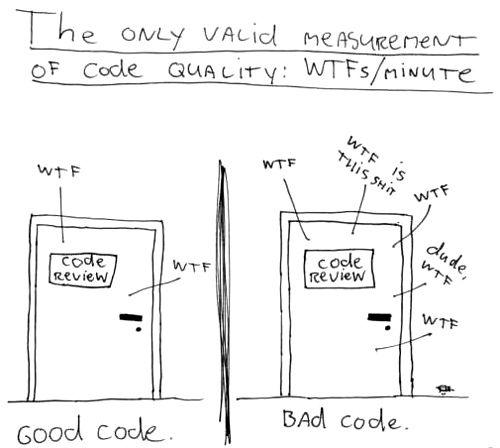
\includegraphics[width=0.65\textwidth]{figs/wtf}
\end{figure}
\end{frame}
%----------------------------FRAME------------------------------------
\begin{frame}[fragile]\frametitle{Coding in Science}
\begin{itemize}

    \item Things should be clever, but not too clever.
    \item Algorithms are optimal, both in speed as well as in readability.
    \item Classes, variables and functions are well named and make sense without having to think too much.
    \item You come back to it after a weekend off, and you can jump straight in.
    \item Things that will be reused are reusable.
    \item Write automated test cases
    \item Unit tests are easy to write.
\end{itemize}
\end{frame}
%----------------------------FRAME------------------------------------
\begin{frame}[fragile]\frametitle{Coding in Science}
%-------------------------------CODE
\begin{minted}[bgcolor=mybg,frame=lines,mathescape]{python}
def p(n):
    """print 3.1415   """
    return n**2
exec(p.__doc__) # hidd
\end{minted}
\begin{minted}[bgcolor=mybg,frame=lines,mathescape]{python}
3.1415
\end{minted}

%-------------------------------END CODE
\end{frame}


% subsection Optimization (end)


\subsection{Profiling your code} % (fold)
\label{sub:Profiling your code}

%----------------------------FRAME------------------------------------
\begin{frame}[fragile]\frametitle{Code profiling}

\begin{block}{timeit (only in ipython)}
\begin{minted} [bgcolor=mybg,frame=lines,bgcolor=mybg,frame=lines,bgcolor=mybg,frame=lines,mathescape]{python}
In [1]: import numpy as np

In [2]: a = np.arange(1000)

In [3]: %timeit a ** 2
100000 loops, best of 3: 5.73 us per loop

In [4]: %timeit a ** 2.1
1000 loops, best of 3: 154 us per loop

In [5]: %timeit a * a
100000 loops, best of 3: 5.56 us per loop
\end{minted}

%-------------------------------END CODE

\end{block}

\end{frame}

%----------------------------FRAME------------------------------------
\begin{frame}[fragile]\frametitle{Profiler}
This is very useful for large programs.
\begin{minted} [bgcolor=mybg,frame=lines,bgcolor=mybg,frame=lines,bgcolor=mybg,frame=lines,mathescape]{python}
# For this example to run, you also need the 'ica.py' file

import numpy as np
from scipy import linalg
from ica import fastica

def test():
    data = np.random.random((5000, 100))
    u, s, v = linalg.svd(data)
    pca = np.dot(u[:10, :], data) 
    results = fastica(pca.T, whiten=False)
test()
\end{minted}

\end{frame}
%----------------------------FRAME------------------------------------
\begin{frame}[fragile]\frametitle{Profiler \%run -t}
\begin{minted} [bgcolor=mybg,frame=lines,bgcolor=mybg,frame=lines,bgcolor=mybg,frame=lines,mathescape]{python}
In [1]: %run -t demo.py

IPython CPU timings (estimated):
    User  :    14.3929 s.
    System:   0.256016 s.
\end{minted}


\end{frame}
%----------------------------FRAME------------------------------------
\begin{frame}[fragile]\frametitle{Profiler \%run -p}
\small
\begin{minted} [bgcolor=mybg,frame=lines,bgcolor=mybg,frame=lines,bgcolor=mybg,frame=lines,mathescape]{python}
In [2]: %run -p demo.py

      916 function calls in 14.551 CPU seconds

Ordered by: internal time

ncalls  tottime  percall  cumtime  percall filename:lineno(function)
     1   14.457   14.457   14.479   14.479 decomp.py:849(svd)
     1    0.054    0.054    0.054    0.054 {method 'random_sample' of 'mtrand.RandomState' objects}
     1    0.017    0.017    0.021    0.021 function_base.py:645(asarray_chkfinite)
    54    0.011    0.000    0.011    0.000 {numpy.core._dotblas.dot}
     2    0.005    0.002    0.005    0.002 {method 'any' of 'numpy.ndarray' objects}
\end{minted}

\end{frame}


%----------------------------FRAME------------------------------------
\begin{frame}[fragile]\frametitle{Line profiler}
The Line Profiler tells us from where our code is called! Save this program as demo.py

\begin{minted} [bgcolor=mybg,frame=lines,bgcolor=mybg,frame=lines,bgcolor=mybg,frame=lines,mathescape]{python}
@profile
def test():
    data = np.random.random((5000, 100))
    u, s, v = linalg.svd(data)
    pca = np.dot(u[:10, :], data)
    results = fastica(pca.T, whiten=False)
\end{minted}
\end{frame}
%----------------------------FRAME------------------------------------
\begin{frame}[fragile]\frametitle{Line Profiler}

\tiny
\begin{minted}[bgcolor=mybg,frame=lines,bgcolor=mybg,frame=lines,bgcolor=mybg,frame=lines,mathescape]{bash}
~ $ kernprof.py -l -v demo.py

Wrote profile results to demo.py.lprof
Timer unit: 1e-06 s

File: demo.py
Function: test at line 5
Total time: 14.2793 s

Line #      Hits         Time  Per Hit   % Time  Line Contents
==============================================================
    5                                           @profile
    6                                           def test():
    7         1        19015  19015.0      0.1      data = np.random.random((5000, 100))
    8         1     14242163 14242163.0   99.7      u, s, v = linalg.svd(data)
    9         1        10282  10282.0      0.1      pca = np.dot(u[:10, :], data)
   10         1         7799   7799.0      0.1      results = fastica(pca.T, whiten=False)
\end{minted}
Use this Link to retrieve \href{http://packages.python.org/line_profiler/kernprof.py}{Kernprof.py (http://packages.python.org/line\_profiler/kernprof.py)}
\end{frame}


\subsection{Speeding your code} % (fold)
\label{sub:Speeding your code}
%----------------------------FRAME------------------------------------
\begin{frame}[fragile]\frametitle{Speed up you code}
Some commonly encountered tricks to make code faster.
\begin{itemize}
    \item Vectorizing for loops \\
     \emph{Avoid for loops} using numpy arrays. For this, masks and indices arrays can be useful.
    \item Broadcasting \\
     Use broadcasting to do operations on arrays as small as possible before combining them
    \item In place operations:
\begin{minted} [bgcolor=mybg,frame=lines,bgcolor=mybg,frame=lines,bgcolor=mybg,frame=lines,mathescape]{python}
In [1]: a = np.zeros(1e7)

In [2]: %timeit global a ; a = 0*a
10 loops, best of 3: 111 ms per loop

In [3]: %timeit global a ; a *= 0
10 loops, best of 3: 48.4 ms per loop

\end{minted}
\end{itemize}
\end{frame}


%----------------------------FRAME------------------------------------
\begin{frame}[fragile]\frametitle{Speed up your code}
\begin{itemize}
    \item Use views, and not copies. \\
    Copying big arrays is as costly as making simple numerical operations on them:
\begin{minted} [bgcolor=mybg,frame=lines,bgcolor=mybg,frame=lines,bgcolor=mybg,frame=lines,mathescape]{python}
In [1]: a = np.zeros(1e7)

In [2]: %timeit a.copy()
10 loops, best of 3: 124 ms per loop

In [3]: %timeit a + 1
10 loops, best of 3: 112 ms per loop
\end{minted}

\end{itemize}
\end{frame}


%----------------------------FRAME------------------------------------
\begin{frame}[fragile]\frametitle{Speed up your code}
Memory access is cheaper when it is grouped: accessing a big array in a continuous way is much faster than random acces. C or Fortran ordering has a strong effect on matrix access.\\
This example is really nice:
\begin{minted} [bgcolor=mybg,frame=lines,bgcolor=mybg,frame=lines,bgcolor=mybg,frame=lines,mathescape]{python}
In [1]: c = np.zeros((1e4, 1e4), order='C')

In [2]: %timeit c.sum(axis=0)
1 loops, best of 3: 3.89 s per loop

In [3]: %timeit c.sum(axis=1)
1 loops, best of 3: 188 ms per loop

In [4]: c.strides
Out[4]: (80000, 8)
\end{minted}
\end{frame}



% subsection Speeding your code (end)

%----------------------------FRAME------------------------------------
\begin{frame}[fragile]\frametitle{Challenge JUN}
\href{https://www.dropbox.com/s/0bvyrc1zf5x1hhk/jun.txt}{https://www.dropbox.com/s/0bvyrc1zf5x1hhk/jun.txt}
\tiny 
\begin{minted} [bgcolor=mybg,frame=lines,bgcolor=mybg,frame=lines,bgcolor=mybg,frame=lines,mathescape]{python}
GACATCATGGGCTATTTTTAGGGGTTGACTGGTAGCAGATAAGTGTTGAGCTCGGGCTGGATAAGGGCTC
AGAGTTGCACTGAGTGTGGCTGAAGCAGCGAGGCGGGAGTGGAGGTGCGCGGAGTCAGGCAGACAGACAG
ACACAGCCAGCCAGCCAGGTCGGCAGTATAGTCCGAACTGCAAATCTTATTTTCTTTTCACCTTCTCTCT
AACTGCCCAGAGCTAGCGCCTGTGGCTCCCGGGCTGGTGTTTCGGGAGTGTCCAGAGAGCCTGGTCTCCA
GCCGCCCCCGGGAGGAGAGCCCTGCTGCCCAGGCGCTGTTGACAGCGGCGGAAAGCAGCGGTACCCACGC
GCCCGCCGGGGGAAGTCGGCGAGCGGCTGCAGCAGCAAAGAACTTTCCCGGCTGGGAGGACCGGAGACAA
GTGGCAGAGTCCCGGAGCCAACTTTTGCAAGCCTTTCCTGCGTCTTAGGCTTCTCCACGGCGGTAAAGAC
CAGAAGGCGGCGGAGAGCCACGCAAGAGAAGAAGGACGTGCGCTCAGCTTCGCTCGCACCGGTTGTTGAA
CTTGGGCGAGCGCGAGCCGCGGCTGCCGGGCGCCCCCTCCCCCTAGCAGCGGAGGAGGGGACAAGTCGTC
GGAGTCCGGGCGGCCAAGACCCGCCGCCGGCCGGCCACTGCAGGGTCCGCACTGATCCGCTCCGCGGGGA
GAGCCGCTGCTCTGGGAAGTGAGTTCGCCTGCGGACTCCGAGGAACCGCTGCGCACGAAGAGCGCTCAGT
GAGTGACCGCGACTTTTCAAAGCCGGGTAGCGCGCGCGAGTCGACAAGTAAGAGTGCGGGAGGCATCTTA
ATTAACCCTGCGCTCCCTGGAGCGAGCTGGTGAGGAGGGCGCAGCGGGGACGACAGCCAGCGGGTGCGTG
CGCTCTTAGAGAAACTTTCCCTGTCAAAGGCTCCGGGGGGCGCGGGTGTCCCCCGCTTGCCACAGCCCTG
TTGCGGCCCCGAAACTTGTGCGCGCAGCCCAAACTAACCTCACGTGAAGTGACGGACTGTTCTATGACTG
CAAAGATGGAAACGACCTTCTATGACGATGCCCTCAACGCCTCGTTCCTCCCGTCCGAGAGCGGACCTTA
TGGCTACAGTAACCCCAAGATCCTGAAACAGAGCATGACCCTGAACCTGGCCGACCCAGTGGGGAGCCTG
AAGCCGCACCTCCGCGCCAAGAACTCGGACCTCCTCACCTCGCCCGACGTGGGGCTGCTCAAGCTGGCGT
CGCCCGAGCTGGAGCGCCTGATAATCCAGTCCAGCAACGGGCACATCACCACCACGCCGACCCCCACCCA
GTTCCTGTGCCCCAAGAACGTGACAGATGAGCAGGAGGGCTTCGCCGAGGGCTTCGTGCGCGCCCTGGCC
GAACTGCACAGCCAGAACACGCTGCCCAGCGTCACGTCGGCGGCGCAGCCGGTCAACGGGGCAGGCATGG
...
\end{minted}
\end{frame}
\begin{frame}[fragile]\frametitle{Challenge JUN (continued)}
\tiny 
\begin{minted} [bgcolor=mybg,frame=lines,bgcolor=mybg,frame=lines,bgcolor=mybg,frame=lines,mathescape]{python}
...
TGGCTCCCGCGGTAGCCTCGGTGGCAGGGGGCAGCGGCAGCGGCGGCTTCAGCGCCAGCCTGCACAGCGA
GCCGCCGGTCTACGCAAACCTCAGCAACTTCAACCCAGGCGCGCTGAGCAGCGGCGGCGGGGCGCCCTCC
TACGGCGCGGCCGGCCTGGCCTTTCCCGCGCAACCCCAGCAGCAGCAGCAGCCGCCGCACCACCTGCCCC
AGCAGATGCCCGTGCAGCACCCGCGGCTGCAGGCCCTGAAGGAGGAGCCTCAGACAGTGCCCGAGATGCC
CGGCGAGACACCGCCCCTGTCCCCCATCGACATGGAGTCCCAGGAGCGGATCAAGGCGGAGAGGAAGCGC
ATGAGGAACCGCATCGCTGCCTCCAAGTGCCGAAAAAGGAAGCTGGAGAGAATCGCCCGGCTGGAGGAAA
AAGTGAAAACCTTGAAAGCTCAGAACTCGGAGCTGGCGTCCACGGCCAACATGCTCAGGGAACAGGTGGC
ACAGCTTAAACAGAAAGTCATGAACCACGTTAACAGTGGGTGCCAACTCATGCTAACGCAGCAGTTGCAA
ACATTTTGAAGAGAGACCGTCGGGGGCTGAGGGGCAACGAAGAAAAAAAATAACACAGAGAGACAGACTT
GAGAACTTGACAAGTTGCGACGGAGAGAAAAAAGAAGTGTCCGAGAACTAAAGCCAAGGGTATCCAAGTT
GGACTGGGTTGCGTCCTGACGGCGCCCCCAGTGTGCACGAGTGGGAAGGACTTGGCGCGCCCTCCCTTGG
CGTGGAGCCAGGGAGCGGCCGCCTGCGGGCTGCCCCGCTTTGCGGACGGGCTGTCCCCGCGCGAACGGAA
CGTTGGACTTTTCGTTAACATTGACCAAGAACTGCATGGACCTAACATTCGATCTCATTCAGTATTAAAG
GGGGGAGGGGGAGGGGGTTACAAACTGCAATAGAGACTGTAGATTGCTTCTGTAGTACTCCTTAAGAACA
CAAAGCGGGGGGAGGGTTGGGGAGGGGCGGCAGGAGGGAGGTTTGTGAGAGCGAGGCTGAGCCTACAGAT
GAACTCTTTCTGGCCTGCCTTCGTTAACTGTGTATGTACATATATATATTTTTTAATTTGATGAAAGCTG
ATTACTGTCAATAAACAGCTTCATGCCTTTGTAAGTTATTTCTTGTTTGTTTGTTTGGGTATCCTGCCCA
GTGTTGTTTGTAAATAAGAGATTTGGAGCACTCTGAGTTTACCATTTGTAATAAAGTATATAATTTTTTT
ATGTTTTGTTTCTGAAAATTCCAGAAAGGATATTTAAGAAAATACAATAAACTATTGGAAAGTACTCCCC
TAACCTCTTTTCTGCATCATCTGTAGATACTAGCTATCTAGGTGGAGTTGAAAGAGTTAAGAATGTCGAT
TAAAATCACTCTCAGTGCTTCTTACTATTAAGCAGTAAAAACTGTTCTCTATTAGACTTTAGAAATAAAT
GTACCTGATGTACCTGATGCTATGGTCAGGTTATACTCCTCCTCCCCCAGCTATCTATATGGAATTGCTT
ACCAAAGGATAGTGCGATGTTTCAGGAGGCTGGAGGAAGGGGGGTTGCAGTGGAGAGGGACAGCCCACTG
AGAAGTCAAACATTTCAAAGTTTGGATTGTATCAAGTGGCATGTGCTGTGACCATTTATAATGTTAGTAG
AAATTTTACAATAGGTGCTTATTCTCAAAGCAGGAATTGGTGGCAGATTTTACAAAAGATGTATCCTTCC
AATTTGGAATCTTCTCTTTGACAATTCCTAGATAAAAAGATGGCCTTTGCTTATGAATATTTATAACAGC
ATTCTTGTCACAATAAATGTATTCAAATACCAA
\end{minted}
\end{frame}

%----------------------------FRAME------------------------------------
\begin{frame}[fragile]\frametitle{Challenge}
\begin{block}{JUN TF gene}
From the above gene, write a code that counts: 
\begin{itemize}
    \item Nuclotide frequency table.
    \item BiNucleotide frequency table. 
    \item TriNucleotide frequency table. 
\end{itemize}
Split your code in several functions. Use the profiler and line profiler to measure the performance of your code. \\
How much your code would spend to process the complete human genome ($3.5\cdot 10^9$ Nucleotides)?
\end{block}



\end{frame}

% subsection Profiling your code (end)


\section{SymPy}
\subsection{First Steps with SimPy} % (fold)
\label{sub:First Steps with SimPy}
%----------------------------FRAME------------------------------------
\begin{frame}[fragile]\frametitle{Symbolic Mathematics in Python}

\begin{block}{Sympy}
SymPy is a Python library for symbolic mathematics. Implements a computer algebra system comparable with Mathematica or Maple.\\
It has a separate website at \href{http://sympy.org}{http://sympy.org}
\end{block}
Capabilities:
\begin{itemize}
    \item Evaluate expressions with arbitrary precision.
    \item Perform algebraic manipulations on symbolic expressions.
    \item Perform basic calculus with symbolic expressions including limits, differentiation and integration.
    \item Solve polynomial and transcendental equations.
    \item Solve some differential equations.
\end{itemize}
\end{frame}

%----------------------------FRAME------------------------------------
\begin{frame}[fragile]\frametitle{Introduction}
\begin{block}{Rational class}
SymPy offers the representation of a Rational class as a pair of two integers, so:
%-------------------------------CODE
\begin{minted}[bgcolor=mybg,frame=lines,mathescape]{python}
>>> from sympy import *
>>> r = Rational(1,2)
>>> r
1/2
>>> r.evalf()
0.500000000000000
\end{minted}

%-------------------------------END CODE
\end{block}

\end{frame}
%----------------------------FRAME------------------------------------
\begin{frame}[fragile]\frametitle{Introduction}
\begin{block}{mpmath}
SymPy uses \href{http://code.google.com/p/mpmath/}{mpmath}. \\ 
Mpmath is a pure-Python library for multiprecision floating-point arithmetic. It provides an extensive set of transcendental functions ($f(x)=x^\pi$), unlimited exponent sizes, complex numbers, interval arithmetic, numerical integration and differentiation, root-finding, linear algebra, and much more. \\
This allows to perform computations using arbitraty precision atithmetic, including the evaluation of $e$, $\pi$, and the inclusion of $\infty$ as a symbol itself through the $oo$. 
\end{block}
\end{frame}

\begin{frame}[fragile]\frametitle{Introduction}

%-------------------------------CODE
\begin{minted}[bgcolor=mybg,frame=lines,mathescape]{python}
>>> pi**2
pi**2
>>> pi.evalf()
3.14159265358979
>>> pi.evalf(60)
3.14159265358979323846264338327950288419716939937510582097494
>>> oo > 10000
True
>>> oo+10000
oo
\end{minted}

%-------------------------------END CODE
\end{frame}

%----------------------------FRAME------------------------------------
\begin{frame}[fragile]\frametitle{Challenge}
\begin{block}{2 mins challenge}
\begin{itemize}
    \item Create two rationals corresponding to $1/2$ and $2/3$ and sum them. 
    \item  Compute the value of $\sqrt{2 \pi \over 3}$ with 30 decimals.   
\end{itemize}
\end{block}

\end{frame}

%----------------------------FRAME------------------------------------
\begin{frame}[fragile]\frametitle{Symbols}
Symbolic variables must be declared explicitly. 
%-------------------------------CODE
\begin{minted}[bgcolor=mybg,frame=lines,mathescape]{python}
>>> from sympy import *
>>> x = Symbol('x')
>>> y = Symbol('y')
\end{minted}

%-------------------------------END CODE
And then comes the magic:
%-------------------------------CODE
\begin{minted}[bgcolor=mybg,frame=lines,mathescape]{python}
>>> x-y+x-y-x+y+y
x
\end{minted}

%-------------------------------END CODE
\end{frame}

% subsection First Steps with SimPy (end)
\subsection{Algebraic manipulations} % (fold)
\label{sub:Algebraic manipulations}
%----------------------------FRAME------------------------------------
\begin{frame}[fragile]\frametitle{Expand}
Expand expands powers and multiplications: 
%-------------------------------CODE
\begin{minted}[bgcolor=mybg,frame=lines,mathescape]{python}
>>> (x+y)**2
(x + y)**2
>>> expand((x+y)**2)
x**2 + 2*x*y + y**2
>>> expand((x)**2, complex=True)
-im(x)**2 + 2*I*im(x)*re(x) + re(x)**2
>>> expand(cos(x+y), trig=True)
-sin(x)*sin(y) + cos(x)*cos(y)
\end{minted}

%-------------------------------END CODE
\end{frame}


%----------------------------FRAME------------------------------------
\begin{frame}[fragile]\frametitle{Simplify}
\begin{block}{simplify()}
%-------------------------------CODE
\begin{minted}[bgcolor=mybg,frame=lines,mathescape]{python}
>>> simplify((x+x*y)/x)
y + 1
\end{minted}

%-------------------------------END CODE
There are specific targeted simplify functions:
\begin{description}
    \item[powsimp] Simplification  of exponents.
    \item[trigsimp] Trigonometric expressions.
    \item[logcombine] $\log(x)+\log(y) = \log(xy)$ and $a \log(x) = \log(x^a)$
    \item[radsimp] Rationalize the denominator.
    \item[together] Rational expressions (\emph{No heroic measures are taken to minimize degree of the resulting numerator and denominator.}, sic.)
    
\end{description}
\end{block}

\end{frame}

%----------------------------FRAME------------------------------------
\begin{frame}[fragile]\frametitle{challenge}
\begin{block}{2 min challenge}

\begin{itemize}
    \item Compute the expanded form of $(x+xy)^3$
    \item Simplify the expression $\sin(x) \over \cos(x)$
\end{itemize}

\end{block}

\end{frame}





% subsection Algebraix manipulations (end)

\subsection{Calculus} % (fold)
\label{sub:Calculus}

%----------------------------FRAME------------------------------------
\begin{frame}[fragile]\frametitle{Limits}
Interestingly, limits are very easy to use in SymPy, just use the sintax:
\begin{block}{limits}
limit(function, variable, point)
\end{block}
\end{frame}

%----------------------------FRAME------------------------------------
\begin{frame}[fragile]\frametitle{Limits}
%-------------------------------CODE
\begin{minted}[bgcolor=mybg,frame=lines,mathescape]{python}
>>> x = Symbol('x')
>>> limit(sin(x)/x, x, 0)
1
>>> limit(x, x, oo)
oo
>>> limit(1/x, x, oo)
0
>>> limit(x**x, x, 0)
1
\end{minted}

%-------------------------------END CODE
\end{frame}

%----------------------------FRAME------------------------------------
\begin{frame}[fragile]\frametitle{Differentiation}

You can differentiate any SymPy expression using:

\begin{block}{differentiation}
diff(func,var,n)
\end{block}

\end{frame}

%----------------------------FRAME------------------------------------
\begin{frame}[fragile]\frametitle{Differentiation}
%-------------------------------CODE
\begin{minted}[bgcolor=mybg,frame=lines,mathescape]{python}
>>> x = Symbol('x')
>>> diff(sin(x), x)
cos(x)
>>> diff(sin(2*x), x)
2*cos(2*x)
>>> diff(tan(x), x)
tan(x)**2 + 1
>>> diff(sin(2*x), x, 3)
-8*cos(2*x)
\end{minted}

%-------------------------------END CODE

\end{frame}
%----------------------------FRAME------------------------------------
\begin{frame}[fragile]\frametitle{Series Expansion}
SymPy also knows how to compute the Taylor series of an expression at a point. Use :
\begin{block}{series}
series(expr,var)
\end{block}
%-------------------------------CODE
\begin{minted}[bgcolor=mybg,frame=lines,mathescape]{python}
>>> x = Symbol('x')
>>> series(cos(x), x)
1 - x**2/2 + x**4/24 + O(x**6)
\end{minted}

%-------------------------------END CODE

\end{frame}


%----------------------------FRAME------------------------------------
\begin{frame}[fragile]\frametitle{Integration}
\begin{block}{Integration}
SymPy has support for indefinite and definite integration of transcendental elementary and special functions via integrate() facility, which uses powerful extended Risch-Norman algorithm and some heuristics and pattern matching.
\end{block}
%-------------------------------CODE
\begin{minted}[bgcolor=mybg,frame=lines,mathescape]{python}
>>> x = Symbol('x')
>>> integrate(2*x**4,x)
2*x**5/5
>>> integrate(cos(x),x)
sin(x)
>>> integrate(log(x)*x,x)
x**2*log(x)/2 - x**2/4
>>> integrate(log(x)*x,(x,0,1))
-1/4
\end{minted}

%-------------------------------END CODE
\end{frame}



% subsection Calculus (end)
\subsection{Equation solving} % (fold)
\label{sub:Equation solving}
%----------------------------FRAME------------------------------------
\begin{frame}[fragile]\frametitle{Solver}

SymPy is able to solve algebraic equations, in one and several variables:
%-------------------------------CODE
\begin{minted}[bgcolor=mybg,frame=lines,mathescape]{python}
>>> x = Symbol('x')
>>> y = Symbol('y')
>>> solve(x**4 - 1, x)
[1, -1, -I, I]
>>> solve([x + 5*y - 2, -3*x + 6*y - 15], [x, y])
{x: -3, y: 1}
>>> solve(exp(x) + 1, x)
[I*pi]
\end{minted}

%-------------------------------END CODE

\end{frame}

%----------------------------FRAME------------------------------------
\begin{frame}[fragile]\frametitle{Factor}
For solving polinomials, also consider the use of \verb|factor|:
%-------------------------------CODE
\begin{minted}[bgcolor=mybg,frame=lines,mathescape]{python}
>>> x = Symbol('x')
>>> f = x**4 - 3*x**2 + 1
>>> factor(f)
(x**2 - x - 1)*(x**2 + x - 1)
\end{minted}

%-------------------------------END CODE
\end{frame}

%----------------------------FRAME------------------------------------
\begin{frame}[fragile]\frametitle{Challenge}
\begin{block}{2 mins challenge}
Could you solve the system of equations: 
\begin{align}
    x+y&=2 \\
    2x+y &= 0
\end{align}
\end{block}

\end{frame}


% subsection Equation solving (end)

\subsection{Linear Algebra} % (fold)
\label{sub:Linear Algebra}
%----------------------------FRAME------------------------------------
\begin{frame}[fragile]\frametitle{Matrix support}
Matrices can be created as instances from the Matrix class: 
%-------------------------------CODE
\begin{minted}[bgcolor=mybg,frame=lines,mathescape]{python}
>>> from sympy import Matrix
>>> Matrix([[1,0],[0,1]])
[1, 0]
[0, 1]
\end{minted}

%-------------------------------END CODE
But... 
%-------------------------------CODE
\begin{minted}[bgcolor=mybg,frame=lines,mathescape]{python}
>>> A = Matrix([[1,x],[y,1]])
>>> A.det()
-x*y + 1
>>> A**2
[x*y + 1,     2*x]
[    2*y, x*y + 1]
\end{minted}

%-------------------------------END CODE
\end{frame}

%----------------------------FRAME------------------------------------
%\begin{frame}[fragile]\frametitle{Differential Equations}
%----------------------------FRAME------------------------------------
%SymPy is capable of solving (some) Ordinary Differential Equations through sympy.ode :
%-------------------------------CODE
%<<term=TRUE,echo=TRUE,fig=FALSE>>=
%from sympy.ode import dsolve
%eq=f(x).diff(x, x) + f(x)
%dsolve(f(x).diff(x, x) + f(x), f(x))
%
%-------------------------------END CODE


%\end{frame}


% subsection Linear Algebra (end)

%----------------------------FRAME------------------------------------
\begin{frame}[fragile]\frametitle{Challenge}
\begin{block}{Differential Equations}
Create a Generic function $f$
%-------------------------------CODE
\begin{minted}[bgcolor=mybg,frame=lines,mathescape]{python}
>>> f = Function("f")
>>> f(x)
f(x)
>>> f(x).diff()
Derivative(f(x), x)
>>> e = Eq( f(x).diff(x,x) + 9*f(x) , 0)
>>> e
9*f(x) + Derivative(f(x), x, x) == 0
>>> dsolve(e,f(x))
f(x) == C1*cos(3*x) + C2*sin(3*x)
\end{minted}

%-------------------------------END CODE

\end{block}

\end{frame}


%----------------------------FRAME------------------------------------
\begin{frame}\frametitle{Questions}
\begin{figure}[!htb]
    \centering
    
\includegraphics[width=0.6\textwidth]{figs/question}
\end{figure}
\end{frame}


\end{document}
